%% Sylhet SOC manuscript -- REVISION v2 (post Soil Security rejection)
%% Reframed around statistically supported findings. Journal-neutral (decide later).
%% Citation Style: elsarticle-harv (Author-Year, Harvard)
%%
%% MARKERS:
%%   [AUTHOR INPUT: ...]  -> needs information only the authors have
%%   LST: DONE -- real Landsat thermal LST extracted (REVISION/lst_real_1985_2025.csv):
%%        +0.66 C/decade, p=0.001, 1988-2025 mean 27.4 C. (Old "+4 C/32 C" was a data artifact.)
%%   Corrected numbers/stats sourced from REVISION/recompute_numbers.py
%%
\documentclass[preprint,authoryear,12pt]{elsarticle}

\usepackage{amsmath}
\usepackage{amssymb}
\usepackage{graphicx}
\usepackage{float}
\usepackage{hyperref}
\usepackage{textcomp}
\usepackage{newunicodechar}
\usepackage{lineno}
\newunicodechar{−}{-}
\usepackage{geometry}
\geometry{margin=1in}
\linenumbers

\journal{Journal of Environmental Management}

\begin{document}
\begin{frontmatter}

\title{Soil Organic Carbon under Warming, Drying and Agricultural Intensification: Integrating Field Sampling, Multi-decadal Remote Sensing and Reanalysis in the Sylhet Haors, Bangladesh}

\author[a]{Md Jashim Uddin\corref{cor1}}
\ead{juswe@du.ac.bd}
\author[a]{Md Rakib Hasan}
\ead{mdrakib-2019417268@swe.du.ac.bd}
\author[a]{Fazla Zawadul Arabi}
\ead{fazlazawadul-2018926633@swe.du.ac.bd}
\author[a]{Anomita Faiz}
\ead{anomita-2019217350@swe.du.ac.bd}
\author[a]{Antara Fairuz}
\ead{antara-2019217251@swe.du.ac.bd}
\author[a]{Arafat Rahman}
\ead{arafat.du.edu@gmail.com}
\cortext[cor1]{Corresponding author}
\affiliation[a]{organization={Department of Soil, Water and Environment, University of Dhaka},
            city={Dhaka}, postcode={1000}, country={Bangladesh}}

\begin{abstract}
Wetlands in South and Southeast Asia are major soil carbon stores, yet they face
intensifying climatic and land-use pressures, and managing them is hampered by sparse field
data and by remote-sensing signals that are easily confounded in seasonally flooded systems.
We present an integrated, multi-source assessment of soil organic carbon (SOC) and its
environmental drivers in nine haor wetlands of the Sylhet Basin, Bangladesh, combining field
soil sampling, multi-decadal satellite remote sensing, climate reanalysis, and external
benchmarking against a global soil database, to derive management-relevant conclusions that no
single data stream could support on its own.
Three data streams with explicitly different temporal scopes were used: a topsoil
geochemical survey (2025 field measurements, with cleaned 1985 reconnaissance-survey
values as an uncertain historical baseline); Landsat-derived vegetation and water
indices (1988--2025); and Sentinel-2 land-use/land-cover (LULC) classification
(2017--2024). Over 2017--2024 the combined open-water plus wetland footprint stayed nearly
constant (coefficient of variation 1.4\%) while the open-water fraction within it swung
2.7-fold between years, indicating that apparent water/flood ``losses'' are seasonal
hydroperiod effects rather than land-use change; the robust LULC signals were a monotonic
$76$\% rise in built-up area ($p=0.002$) and a modest $22$\% vegetation-class decline
($p=0.006$). Dry-season (water-controlled) Landsat composites revealed significant
agricultural intensification and warming over 1988--2025: dry-season NDVI rose
($+0.031$ decade$^{-1}$, Mann--Kendall $p<0.001$; a $+22$\% greening consistent with expanding
irrigated Boro rice) and land surface temperature warmed ($+0.55\,^{\circ}$C decade$^{-1}$,
$p=0.015$). Optical water indices could not resolve a hydrological trend (the annual NDWI signal
is confounded by the seasonal open-water fraction), but independent ERA5-Land reanalysis showed
the basin is also drying---root-zone soil moisture ($-0.033$~m$^3$\,m$^{-3}$ decade$^{-1}$,
$p=0.02$) and precipitation ($-161$~mm decade$^{-1}$, $p=0.02$) both declined over 1985--2025,
with concurrent air-temperature warming ($p<0.001$). In 2025, topsoil SOC showed \emph{no} relationship with clay content ($r=0.04$, $p=0.93$);
soil texture was not a predictor of SOC across sites. Benchmarking against $\sim$9{,}700 profiles
of the same (acidic, clay-rich) soil class in the WoSIS database reproduced this null, whereas
clay does predict SOC modestly across soils globally---indicating that where clay is already
abundant the mineral-associated carbon pool approaches saturation and texture ceases to limit
SOC. SOC instead scaled with organic-matter quantity (indexed by total nitrogen), implying that
inputs and management, not mineral protection, govern carbon storage in these soils. Comparison with the historical baseline indicates a heterogeneous, site-dependent SOC response (six of nine sites
lower in 2025, three higher); the change was not statistically significant (paired $p=0.15$)
and was sensitive to two high-uncertainty baseline values, so it is reported as suggestive
rather than definitive. Together the results depict a wetland system under warming, drying and
agricultural intensification---rather than loss of inundated extent---in which SOC is governed
primarily by site-level land management and organic-matter inputs. We translate these findings
into specific management priorities---sustaining the seasonal flood pulse and organic-matter-returning
rice practices, directing urban expansion away from high-carbon cores, and establishing long-term
soil, temperature and hydroperiod monitoring---and into a transferable, confound-aware framework
for assessing and managing SOC in data-poor South and Southeast Asian wetlands. A central
methodological lesson for wetland management is that inundated-area imagery alone can misrepresent
hydrological change: the basin is warming and drying even though its wet-season footprint appears
stable.
\end{abstract}

\begin{keyword}
soil organic carbon \sep haor wetland \sep hydroperiod \sep Landsat time series \sep
land-use change \sep Boro rice \sep organo-mineral carbon \sep inverse distance weighting \sep Bangladesh
\end{keyword}
\end{frontmatter}

%% ============================================================
\section{Introduction}
\label{sec:introduction}

Wetlands are among the most important ecosystems globally, covering approximately
15--16 million km$^2$, of which about 91\% are inland and 9\% coastal \citep{Davidson2023}.
Despite conservation efforts, natural wetlands declined by about 35\% between 1970 and 2015
while man-made wetlands grew by 233\% \citep{ConventionWetlands2021}. Bangladesh has shared
in this loss; Dhaka alone has lost 69\% of its wetlands \citep{Abdullah2024}.

Wetlands deliver multiple ecosystem services---carbon and nutrient cycling, water-quality
regulation, flood buffering and habitat provision \citep{Lamsal2017}---with a global value
estimated at \$26.4 trillion yr$^{-1}$ \citep{Costanza2014}. They store roughly 20--30\% of
the global soil carbon pool \citep{Nahlik2016} and sequester carbon at 20--30 g C m$^{-2}$
yr$^{-1}$ in freshwater systems \citep{Chmura2003}, principally because prolonged
inundation suppresses microbial decomposition and preserves organic matter (OM)
\citep{Xiaonan2008}. Net carbon accumulation therefore depends strongly on a wetland's
hydrology, and practices that alter that hydrology can release previously stored SOC
\citep{Limpert2020}. In Bangladesh the haor region comprises 373 bowl-shaped depressions
covering about 859{,}000 ha---10\% of national wetland area \citep{Davidson2014,HaorMasterPlan}.
Haors receive monsoon runoff and seasonal inundation, then dry out in winter
\citep{Nishat1993}; they are concentrated in the northeastern Sylhet sub-basin
\citep{Salauddin2010}.

Remote sensing is now central to wetland study, supporting LULC change detection, wetland
mapping, hydrological and vegetation monitoring, and carbon-cycle analysis across space and
time \citep{Schmidt2003,Erener2012}. Multi-temporal imagery has tracked wetland change since
the early 1980s \citep{Papastergiadou2007}, capturing degradation driven by LULC change
\citep{Guo2017}, climate change \citep{Donner2003}, water-table fluctuation \citep{Funk1994}
and urban expansion \citep{Gillies2003,Ramachandra2020}. Three spectral indices are
particularly informative as process proxies in this setting. The Normalized Difference
Vegetation Index (NDVI) tracks green biomass and primary productivity, i.e.\ the
\emph{rate of OM input} to soils \citep{Rouse1973}. The Normalized Difference Water Index
(NDWI) tracks surface and canopy water content \citep{McFeeters1996}, a proxy for the
\emph{anaerobic, decomposition-suppressing conditions} on which wetland carbon storage
depends. The Built-Up Index (BUI) tracks impervious expansion \citep{Zha2003}, a proxy for
\emph{conversion pressure} that alters hydrology and OM inputs. Linking these indices to
field SOC therefore connects the satellite-observable drivers (water availability,
vegetation productivity, urbanization) to the soil-carbon outcome.

This study examines nine haor wetlands of the Sylhet region. Rather than relying on field data
alone---which, as in most data-poor wetlands, are sparse---we develop an integrated assessment
that combines limited field sampling with multiple public Earth-observation and reanalysis
datasets, using each to constrain what the others cannot. Our objectives are to (1) characterize
present-day (2025) topsoil SOC and its geochemical controls across contrasting haor land uses;
(2) quantify recent landscape transformation (LULC 2017--2024) and multi-decadal trends in
warming, hydrology and vegetation (1985/1988--2025); and (3) interpret SOC in relation to these
drivers, benchmarking the field result against a global soil database. The intended contribution
is threefold and is not contingent on the small field sample: a transferable, confound-aware
\emph{framework} for assessing wetland soil carbon where field data are scarce; a
\emph{methodological caution} that inundated-area imagery can misrepresent wetland hydrological
change (so that warming and drying must be read from thermal and reanalysis products, not optical
water indices); and an \emph{externally validated} finding on the controls of SOC in clay-rich
wetland soils, with direct management implications.

We frame two hypotheses, each tested against the data and reported regardless of outcome:

\noindent\textbf{H1:} \textit{Progressive warming, drying and agricultural intensification over
the multi-decadal record (rising temperature, declining soil moisture and rainfall, and
dry-season greening) are associated with SOC decline, because warmer, drier soils and intensified
cultivation (drainage, residue export, tillage) accelerate organic-matter turnover.}

\noindent\textbf{H2:} \textit{Soil clay content governs SOC retention across sites, with
finer-textured soils storing more SOC through organo-mineral protection.}

%% ============================================================
\section{Materials and Methods}
\label{sec:methodology}

\subsection{Study area}
\label{subsec:study-area}
The study area comprises nine lowland haor wetlands of the Sylhet region---Ajmiriganj,
Balaganj, Goainghat, Hakaluki, Kanairghat, Phagu, Sarail, Sulla and Terchibari---spanning a
GIS-delineated boundary of approximately 12{,}300 km$^2$ (Fig.~\ref{fig:study-area}). The region
has a subtropical monsoon climate with heavy rainfall in June--September that drives seasonal
inundation controlling hydrology and vegetation.

\begin{figure}[htbp]\centering
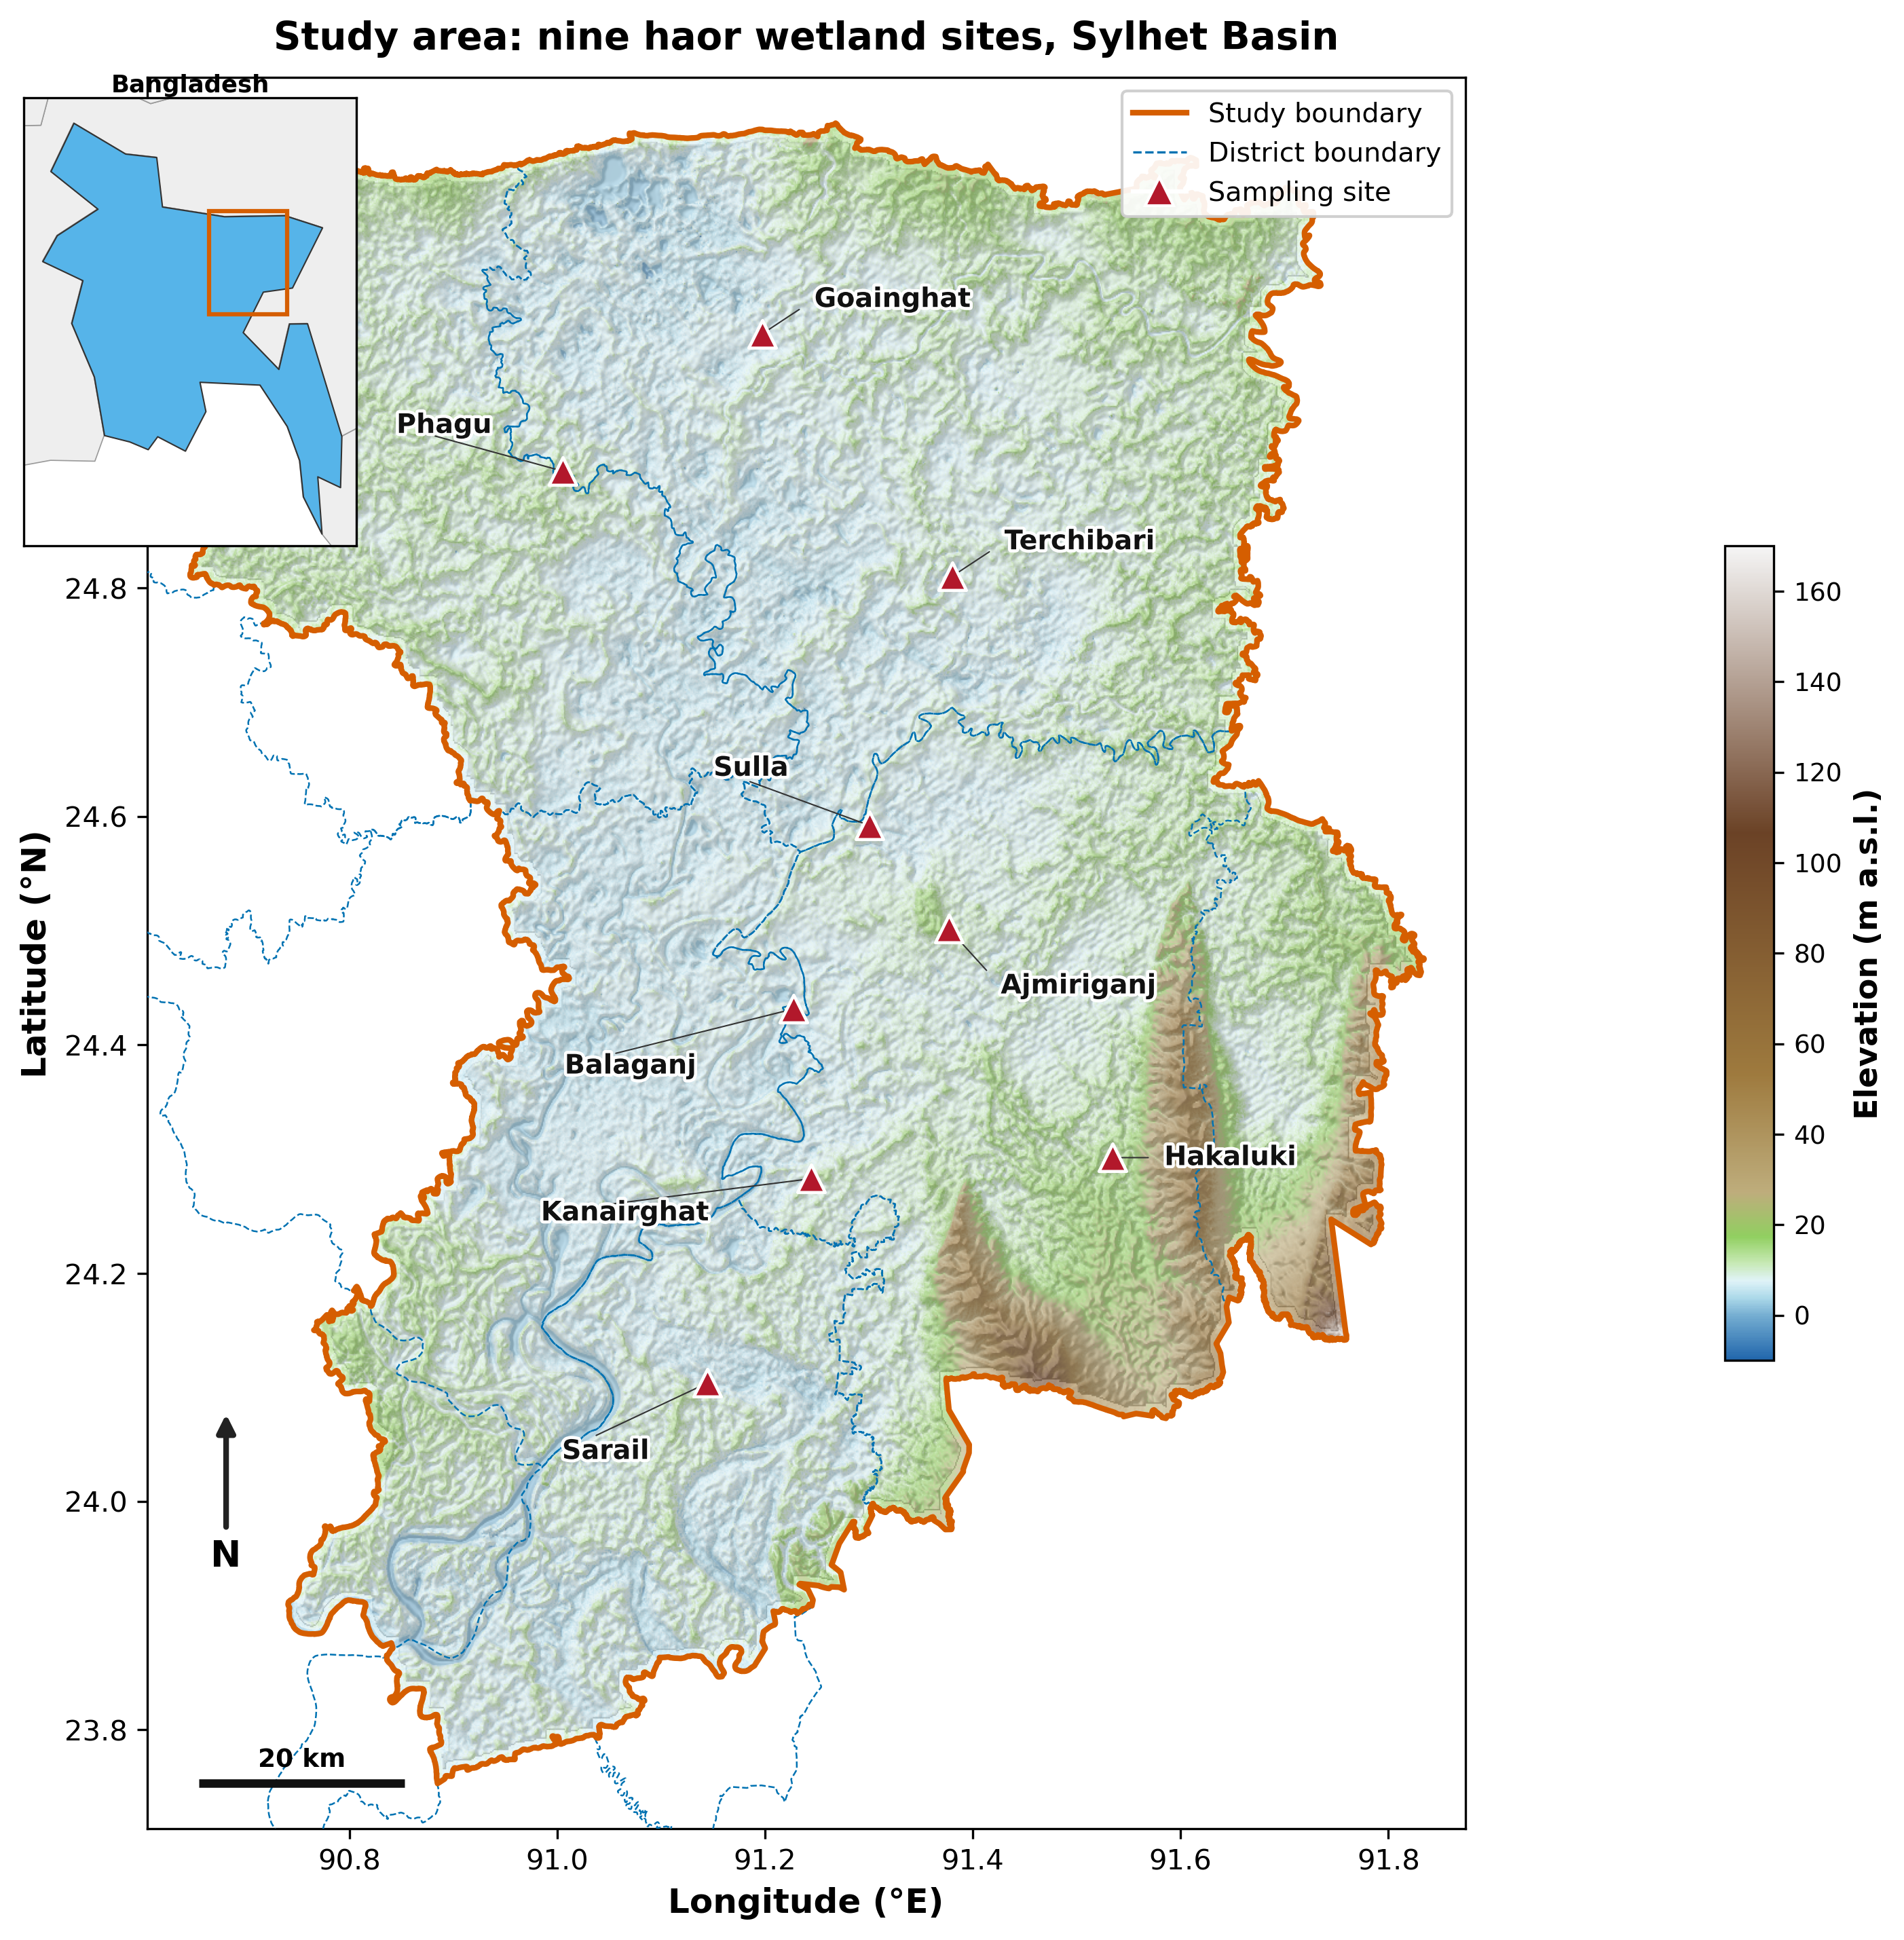
\includegraphics[width=0.7\textwidth]{Fig1_StudyAreaMap.png}
\caption{Study area showing the nine haor sampling sites in the Sylhet Basin, Bangladesh,
over an SRTM elevation backdrop. [Fig 1 to be redrawn: remove/clarify the SOC legend and
resolve overlapping scale bars per reviewer comment 7.]}
\label{fig:study-area}\end{figure}

\subsection{Soil sampling and laboratory analysis}
\label{subsec:soil-analysis}
% Reviewer comments 5, 6, 8, 13 -- methodological transparency.
In 2025, at each of the nine sites a composite topsoil sample (0--30~cm) was collected by
bulking three cores taken within the sampling area, together with a subsoil sample
(30--100~cm); the analysis below focuses on the topsoil (SOCiT). Sampling locations were
georeferenced with a handheld GPS, and samples were transported to the laboratory on the day
of collection. Prior to analysis, samples were air-dried, gently crushed, sieved to 2~mm, and
visible roots and debris removed.

Soil pH was measured potentiometrically (1:2.5 soil:water) following \citet{Jackson1967}.
SOC was determined by Walkley--Black wet oxidation \citep{Walkley1934}, with a recovery-factor
correction of 1.30 (van Bemmelen) applied to account for incomplete oxidation.
Total nitrogen (TN) was
determined by Kjeldahl digestion \citep{Kjeldahl1883}. Particle-size distribution
(clay fraction) was measured by the Bouyoucos hydrometer method \citep{Bouyoucos1936}.
Bulk density (SBD) was measured by the core method \citep{Blake1965}. Cation exchange
capacity (CEC) was determined following \citet{Chapman1965}.

\subsection{Historical (1985) soil baseline and data screening}
\label{subsec:baseline}
% Reviewer E4, comments 5/13; data-quality audit.
Historical topsoil values for the same nine sites were compiled from the Soil Resource
Development Institute (SRDI) Upazila Nirdeshika (Upazila Land and Soil Resource Utilization
Guide) reconnaissance soil-survey series \citep{SRDI_Nirdeshika} to provide a $\sim$1985
baseline. Because these are secondary
reconnaissance data of unknown analytical precision, all baseline values were screened
against physical limits before use. Entries failing basic plausibility were treated as
missing: one pH recorded as 0 (Hakaluki subsoil), and bulk-density values exceeding the
density of quartz, 2.65 g cm$^{-3}$ (Phagu 2.91, Terchibari 2.82 g cm$^{-3}$). Several
further baseline values were flagged as high-uncertainty (topsoil SBD $>$2.0 g cm$^{-3}$ at
five sites; peat-like SOC of 7.01\% and 4.30\% at Hakaluki and Sarail). Because SOC stock
is the product of SOC concentration and bulk density, and the 1985 SBD column is
systematically inflated, we report baseline SOC as \emph{concentration} (directly reported)
and treat baseline \emph{stock} as indicative only. Long-term change is reported with
site-level detail and an outlier-sensitivity analysis (Section~\ref{subsec:soc-change}).

\subsection{SOC stock calculation and spatial interpolation}
\label{subsec:soc-stock}
% Reviewer comments 8, 10, 39.
Topsoil SOC stock was computed as
\begin{equation}
\mathrm{SOC\ stock\ (Mg\ ha^{-1})} = \mathrm{SOC\%} \times \mathrm{SBD\ (g\ cm^{-3})}
\times d\ \mathrm{(cm)} \times 0.1,
\label{eq:stock}
\end{equation}
where $d = 30$~cm is the topsoil sampling depth (SOC\% expressed as a fraction; the factor
0.1 converts to Mg~ha$^{-1}$). Throughout, we report SOCiT (immobilized topsoil SOC stock,
$0$--$30$~cm). The spatial distribution of SOCiT was mapped by Inverse Distance Weighting
(IDW; \citealp{Burrough2015}) after projecting site coordinates to UTM Zone 46N (EPSG:32646),
at 30 m resolution to match Landsat. Note that Fig.~\ref{fig:soc-stock} maps SOCiT (the
quantity discussed in the text), correcting the earlier mismatch between the mapped variable
and the in-text values.

\subsection{Satellite data and processing}
\label{subsec:rs}
Remote-sensing processing used Google Earth Engine (GEE). Three sources were combined:
Landsat Collection-2 Level-2 surface reflectance (Landsat 5 TM, 7 ETM+, 8 OLI; 1985--2024,
30 m) for long-term index trends; Sentinel-2 MSI (2017--2025, 10 m) for LULC classification;
and ESA CCI Above-Ground Biomass for biomass cross-validation. Landsat scenes with $>$90\%
cloud were excluded at scene level and cloudy pixels masked via the QA band; Sentinel-2 was
restricted to $<$10\% scene cloud with an additional NDVI-based residual-cloud mask. NDVI was
computed as (NIR$-$Red)/(NIR$+$Red) (Landsat 5/7 B4,B3; Landsat 8 B5,B4; Sentinel-2 B8,B4);
and NDWI as the McFeeters (Green$-$NIR)/(Green$+$NIR) open-water index \citep{McFeeters1996}
(Landsat 5/7 B2,B4; Landsat 8 B3,B5; Sentinel-2 B3,B8). Because the haors flood seasonally, whole-year mean indices are dominated by the variable open-water
fraction in each year's imagery (annual-mean NDVI and NDWI correlate at $r=-0.89$ across years,
i.e.\ they largely track the same water-fraction artifact). To obtain interpretable vegetation
and temperature trends we therefore computed \emph{dry-season} (February--April; pre-monsoon,
peak-Boro) median composites for each year over the study polygon, when standing water is
minimal. This reduced the open-water fraction to $\sim$1.3\% of the area (with no temporal trend),
effectively decoupling the indices from the seasonal flood pulse; we report NDVI on both the full
composite and over land only (NDWI $<0$), which were nearly identical. Index values outside
$[-1,1]$ were removed. In dry-season composites NDWI carries little hydrological information (it
mirrors NDVI, $r=-0.97$) and is not interpreted as a drying signal.

\subsection{Land surface temperature}
\label{subsec:lst}
% Reviewer comment 32 + audit: the submitted LST column was corrupt.
Land surface temperature (LST) was derived from Landsat Collection-2 Level-2 thermal
surface-temperature bands (ST\_B6 for Landsat 5/7; ST\_B10 for Landsat 8/9), converted to
$^{\circ}$C using the USGS scaling (LST $= \mathrm{ST} \times 0.00341802 + 149.0 - 273.15$),
with QA-band cloud/shadow masking, then averaged over the study boundary at 100 m for the same
dry-season (February--April) window as the vegetation indices.
Thermal data were unavailable for 1985--1987 (insufficient Landsat-5 coverage) and one year
(1992) returned an implausible basin mean ($11.6\,^{\circ}$C, a residual-cloud artifact) and
was excluded, leaving 37 annual values (1988--2025).

\subsection{Independent hydrological reanalysis}
\label{subsec:hydro-data}
Because the optical water index is confounded in this seasonally flooded basin
(Section~\ref{subsec:rs}), we characterised the hydrological trend using three model- and
satellite-based products independent of optical imagery: ERA5-Land reanalysis
\citep{MunozSabater2021}, from which we extracted basin-mean annual root-zone (0--100~cm) soil
moisture, total precipitation, 2~m air temperature and potential evaporation (1985--2025);
GLDAS-2.1 \citep{Rodell2004}, providing an independent root-zone soil moisture and
evapotranspiration (2000--2025); and GRACE/GRACE-FO terrestrial water-storage anomalies
\citep{Tapley2004} (2003--2016). All were aggregated to basin-mean annual series and tested for
trend with Mann--Kendall and Sen's slope.

\subsection{LULC classification and change analysis}
\label{subsec:lulc}
% Reviewer comments 9, 28, 30.
Annual LULC maps (2017--2024, 10 m) were produced from Sentinel-2 MSI in Google Earth Engine
using a supervised Random Forest classifier (an ensemble of decision trees, default
configuration) trained on the Sentinel-2 reflectance bands (B2, B3, B4, B8) together with
derived NDVI and NDWI; training samples were regions of interest digitized by visual
interpretation of high-resolution imagery for each class. Classes were Water, Vegetation, Flood-prone, Urban,
and Flooded vegetation. Classification accuracy was assessed against 285 stratified-random
reference points (about 40 per class) interpreted on high-resolution 2024 satellite imagery.
At the functional level at which we interpret the data---merging the seasonally interconverting
water, flood-prone, flooded-vegetation and wetland categories into a single hydromorphic class
(Section~\ref{subsec:lulc-change})---overall accuracy was 83.2\% (Cohen's $\kappa=0.74$). The
two classes carrying our quantitative trend claims were classified reliably (urban user's
accuracy 95\%, vegetation user's accuracy 98\%), whereas the individual hydromorphic sub-classes
were not separable on single-date imagery because they interconvert with the flood pulse (the
full per-class confusion matrix is given in Table~\ref{tab:confusion}). We therefore restrict
quantitative LULC inference to the urban and vegetation classes and to the aggregated
hydromorphic footprint, and do not interpret transitions among the individual
water/flood/wetland sub-classes.

\begin{table}[htbp]\centering
\caption{Confusion matrix of the 2024 LULC classification against 285 stratified-random
reference points (full eight-class scheme). Rows are reference (true) classes, columns are
mapped (predicted) classes; the final column is producer's accuracy (PA) and the final row
user's accuracy (UA), in \%. Misclassification is confined almost entirely to exchanges among
the hydromorphic sub-classes (water, flood-prone, flooded vegetation, wetland), which
interconvert with the seasonal flood pulse; merging these into one hydromorphic class raises
overall accuracy to 83.2\% ($\kappa=0.74$).}
\label{tab:confusion}
\small\setlength{\tabcolsep}{4pt}
\begin{tabular}{lrrrrrrrr|r}
\hline
true \textbackslash{} pred & Wat & Fld & FlV & Wet & Veg & Urb & Bar & Oth & PA\% \\
\hline
Water              & 13 & 1  & 1  & 0  & 0  & 0  & 2  & 0 & 76 \\
Flood-prone        & 3  & 17 & 0  & 0  & 0  & 0  & 0  & 0 & 85 \\
Flooded vegetation & 9  & 21 & 30 & 40 & 1  & 2  & 4  & 1 & 28 \\
Wetland            & 0  & 0  & 0  & 0  & 0  & 0  & 0  & 0 & -- \\
Vegetation         & 12 & 1  & 2  & 0  & 39 & 0  & 1  & 0 & 71 \\
Urban              & 3  & 0  & 0  & 0  & 0  & 38 & 8  & 3 & 73 \\
Bare/Fallow        & 0  & 0  & 7  & 0  & 0  & 0  & 25 & 1 & 76 \\
Other              & 0  & 0  & 0  & 0  & 0  & 0  & 0  & 0 & -- \\
\hline
UA\%               & 32 & 42 & 75 & -- & 98 & 95 & 62 & -- &    \\
\hline
\end{tabular}
\end{table}

Class areas were extracted per year by pixel counting (each Sentinel-2 pixel = 100 m$^2$).
LULC change was quantified two ways: (i) endpoint difference (2017 vs 2024) and (ii) the
linear and rank (Spearman) trend across all eight years, so that change is not inferred from
two dates alone (reviewer comment 28). Site-scale context was summarized within 500 m buffers
(78.54 ha) around each sampling point.

\subsection{Biomass estimation}
\label{subsec:biomass}
% Reviewer comments 11, 33.
Above-ground biomass (AGB, t ha$^{-1}$ yr$^{-1}$) was estimated from annual NDVI using the
quadratic relationship
\begin{equation}
\mathrm{AGB} = 11.59\,\mathrm{NDVI}^2 - 4.96\,\mathrm{NDVI} + 0.76,
\label{eq:biomass}
\end{equation}
adopted from \citet{Meshesha2020}, who calibrated it against field plots ($n=28$, $R^2=0.81$).
We note this relationship was developed for semi-arid grassland in Ethiopia rather than for
wetland rice systems, so the absolute biomass values should be read as indicative; it is used
here only to summarize the relative temporal NDVI--productivity signal, which is corroborated
by the independent ESA CCI AGB record. The quadratic form captures NDVI saturation in dense
canopies. Estimates were cross-checked against ESA CCI AGB (2010--2021, $\sim$100 m). NDVI-based estimation begins in 1988 because earlier Landsat-5
coverage of the area is too sparse for reliable annual composites.

\subsection{Statistical analysis}
\label{subsec:stats}
% Reviewer comments 2, 20, 31, 36, 38, 40 -- real statistics, with explicit n.
All analyses were based on $n=9$ sites; given this small sample, the multivariate results (PCA,
clustering) were treated as \emph{exploratory}, and we report effect sizes
with exact $p$-values rather than relying on the word ``significant''. Bivariate associations
were quantified as Pearson and Spearman coefficients with $p$-values. Long-term SOC change was
tested with a paired $t$-test and the robust Wilcoxon signed-rank test, together with a
leave-out sensitivity analysis for the two high-uncertainty baseline sites. Multi-decadal index
trends (1988--2025) were assessed with the non-parametric Mann--Kendall test and Sen's slope,
and cross-checked against ordinary least squares; LULC trends (2017--2024) were tested likewise.
The PCA used standardized soil variables, with loadings, eigenvalues and explained variance
tabulated (Table~\ref{tab:pca}). All analyses were performed in Python 3.9 (pandas, NumPy,
SciPy, scikit-learn; \citealp{Pedregosa2011}).

To place the nine-site results in a broader context and test whether the SOC--property relations
generalize beyond our small sample, we benchmarked them against the WoSIS global soil-profile
database \citep{Batjes2020}. WoSIS horizons were depth-weighted to a 0--30~cm topsoil value per
profile (matching our sampling), and a ``Sylhet soil class'' was defined by our sites' predictor
envelope---acidic (pH $<6$) and clay-rich (clay 30--75\%)---rather than by SOC, to avoid
conditioning on the response. Within this class ($n=9{,}676$ global profiles) we recomputed the SOC--property Spearman
correlations and the partial correlation of clay with SOC controlling for nitrogen. To obtain a
genuine land-cover (not merely soil-class) wetland benchmark, we sampled the Copernicus CGLS-LC100
(2019) discrete classification \citep{Buchhorn2020} at each profile in Google Earth Engine and
isolated the cultivated/paddy ($n=2{,}425$) and herbaceous-wetland ($n=96$) subsets. We also
joined WorldClim mean annual temperature and precipitation \citep{Hijmans2005} to each profile
for a space-for-time test of the temperature--SOC relationship (partial correlations and a
standardized log-SOC multiple regression). We note WoSIS is a multi-source compilation of
variable analytical vintage, the land cover is a single recent epoch, and the space-for-time
substitution assumes spatial temperature gradients approximate temporal change, so these
benchmarks are approximate.

%% ============================================================
\section{Results}
\label{sec:results}

\subsection{Present-day SOC and soil geochemistry (2025)}
\label{subsec:soc-2025}
In 2025, topsoil SOC ranged from 0.64\% (Phagu) to 2.63\% (Ajmiriganj), and SOCiT from
30.7 Mg ha$^{-1}$ (Phagu) to 122.7 Mg ha$^{-1}$ (Ajmiriganj) (Fig.~\ref{fig:soil-properties}).
The highest values occurred at Ajmiriganj under irrigated Boro--fallow management, consistent
with reports that continuous flooding plus straw/residue inputs enhance carbon storage in
Asian rice paddies \citep{Chen2021}.
The central result concerns clay: SOC showed \emph{no} association with clay content
($r=0.04$, $p=0.93$; and for every stock metric, $|r|\leq0.21$, $p\geq0.59$). The two
highest-clay sites (Terchibari 72\%, Goainghat 68\%) had among the lowest SOCiT, whereas the
highest-SOCiT site (Ajmiriganj) had intermediate clay. \textbf{Thus H2 is not supported}: across
these nine haors, soil texture does not govern SOC storage. This is consistent with the concept
of mineral-associated organic-matter saturation---where clay is already abundant (here 30--72\%),
additional clay confers little extra protective capacity, so texture ceases to be the limiting
control \citep[e.g.][]{Cotrufo2019,Georgiou2022}. SOC instead co-varied most strongly with total
nitrogen (TN; Pearson $r=0.82$, $p=0.006$) and weakly, non-significantly, with pH ($r=-0.52$,
$p=0.16$). We interpret the SOC--TN relationship cautiously: because soil nitrogen is
predominantly organic and bound within organic matter at a relatively constrained C:N ratio,
SOC and TN are partly coupled by construction, so this association indicates that SOC here is set
by organic-matter \emph{quantity}---i.e.\ by inputs and management---rather than identifying
nitrogen as an independent causal control. The substantive, non-trivial finding is therefore the
\emph{absence} of a clay (texture) control, not the presence of an N control.

Other soil properties behaved as expected for these soils. CEC ranged from 16.7 to 32.5
cmol$_c$ kg$^{-1}$ (a decimal data-entry error in the original laboratory record was corrected)
and scaled strongly with clay ($r=0.93$, $p<0.001$), reflecting the contribution of fine particles
to exchange sites. Bulk density was inversely related to clay
($r=-0.72$, $p=0.028$), consistent with finer soils having greater porosity and lower packing
density. Soils were strongly acidic (pH 4.0--5.9),
consistent with prolonged waterlogging and leaching, and TN was low (0.10--0.15\%).

\begin{figure}[htbp]\centering
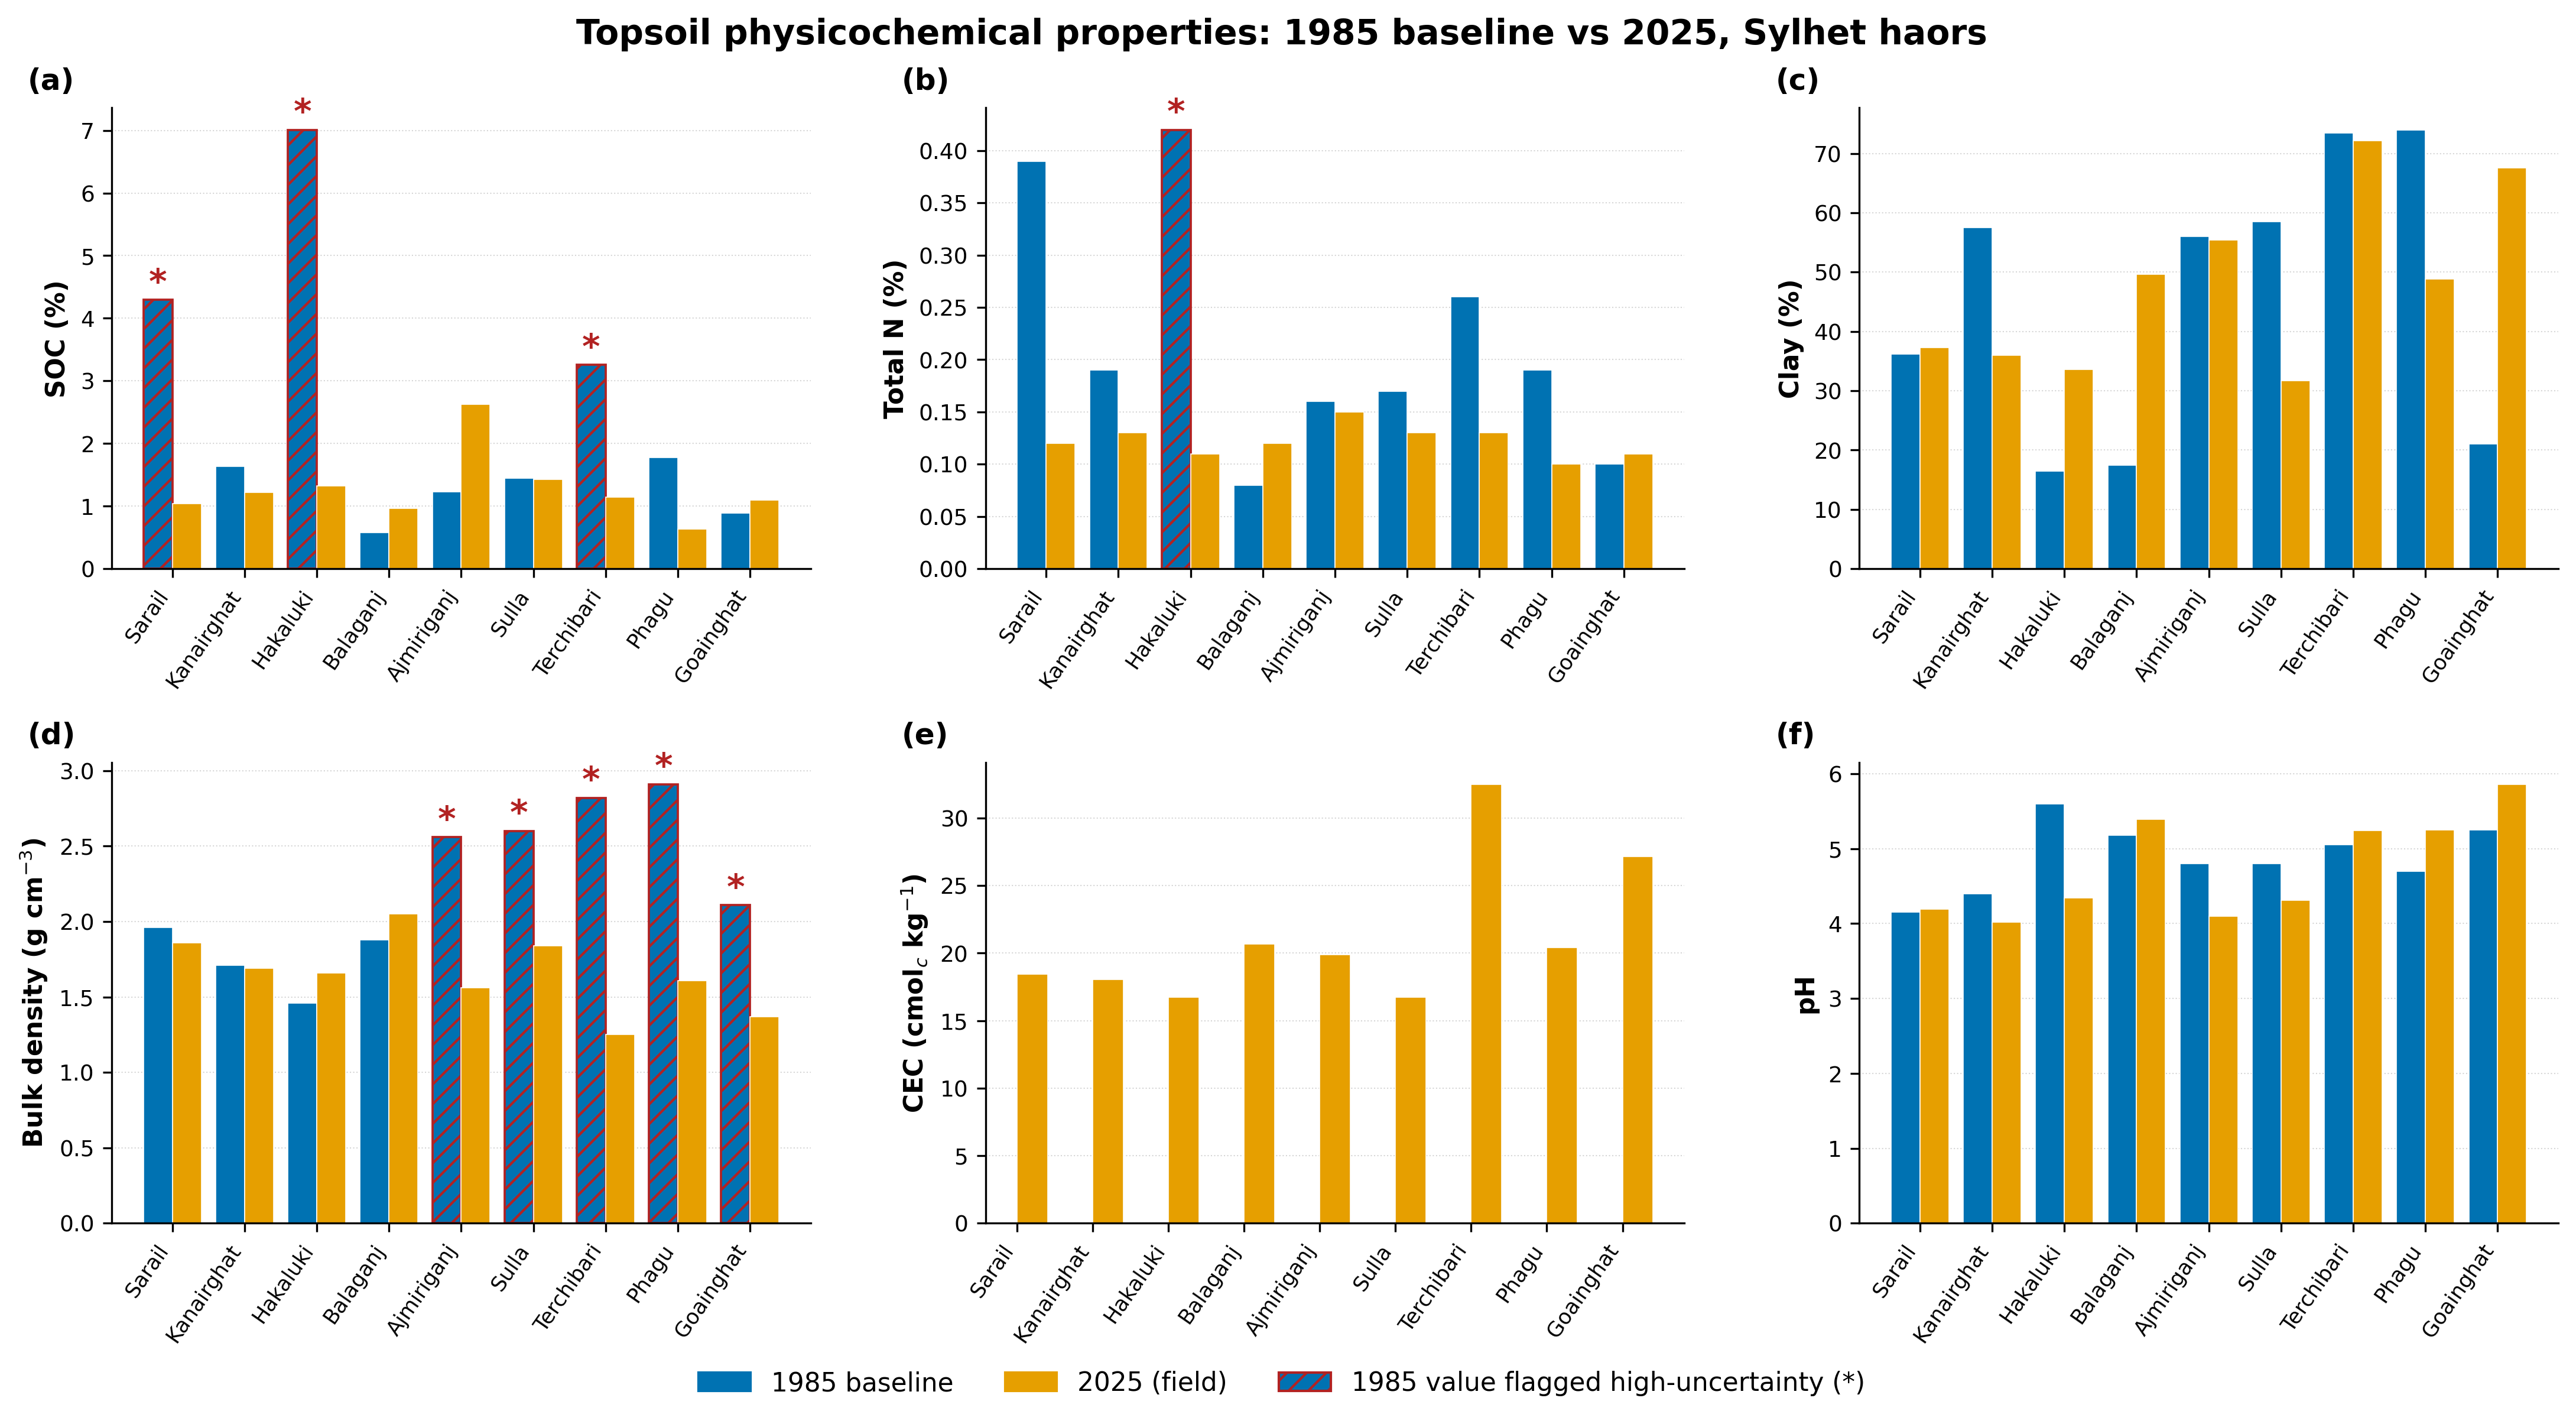
\includegraphics[width=0.75\textwidth]{Fig2_SoilProperties.png}
\caption{Topsoil physicochemical properties (SOC\%, TN, clay, bulk density, CEC, pH) at the
nine sites in 2025, with the cleaned 1985 reconnaissance baseline for reference. Baseline
values flagged as high-uncertainty (Section~\ref{subsec:baseline}) are marked.}
\label{fig:soil-properties}\end{figure}

\subsection{Long-term context: an uncertain historical comparison}
\label{subsec:soc-change}
We treat the 2025 measurements primarily as a present-day snapshot; the comparison with the 1985
SRDI baseline is offered only as cautious historical context, not as a primary result. That
comparison is heterogeneous (six of nine sites lower in 2025, three higher) and \emph{not
statistically significant} (paired $t$-test $p=0.15$; Wilcoxon $p=0.20$); moreover, the apparent
mean decline is dominated by two baseline values flagged as high-uncertainty (peat-like 1985
concentrations of 7.01\% and 4.30\% at Hakaluki and Sarail), and falls from $-$48\% to $-$16\%
when these are excluded. Given single-time-point sampling and a secondary reconnaissance baseline
(Section~\ref{subsec:limitations}), we draw no quantitative conclusion about long-term SOC change;
it is best regarded as a hypothesis motivating the long-term monitoring we recommend below.

\begin{figure}[htbp]\centering
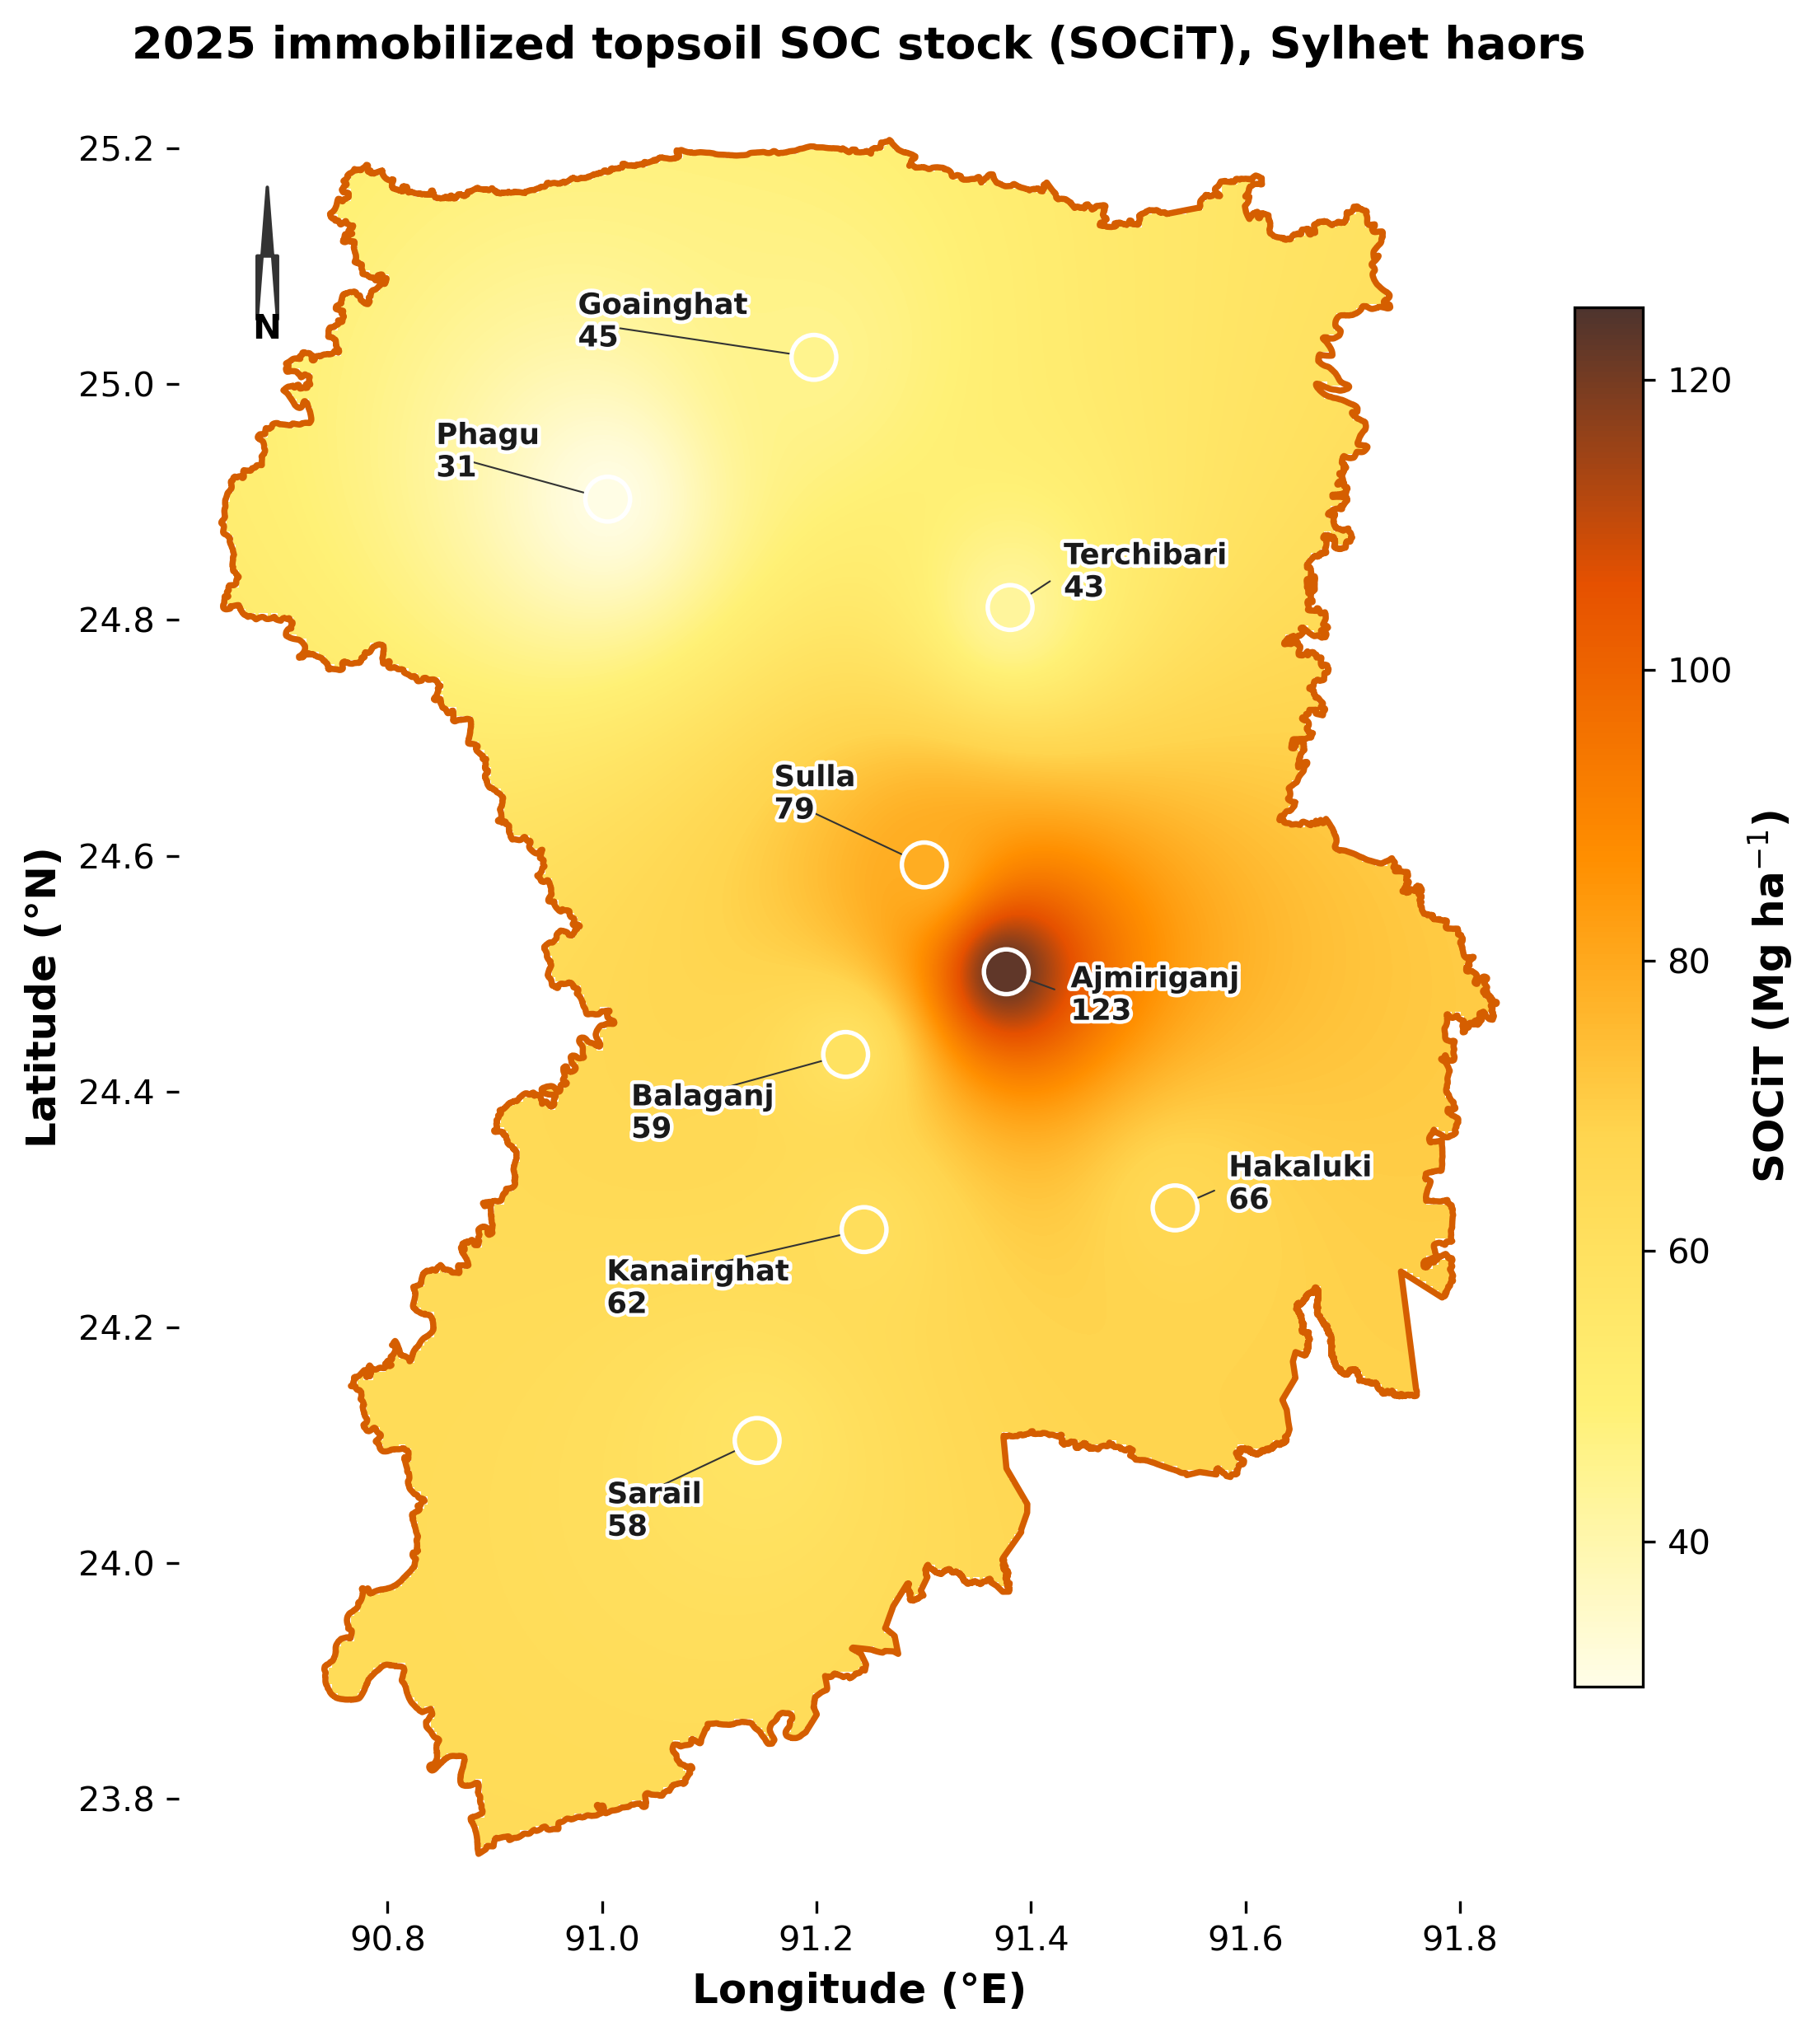
\includegraphics[width=0.8\textwidth]{Fig3_SOCStockMap.png}
\caption{IDW-interpolated immobilized topsoil SOC stock (SOCiT, Mg ha$^{-1}$) across the
Sylhet haors in 2025. (Now mapping SOCiT---the quantity discussed in the text---rather than
total stock; cf.\ reviewer comment 39.)}
\label{fig:soc-stock}\end{figure}

\subsection{Recent landscape transformation (LULC 2017--2024)}
\label{subsec:lulc-change}
Interpreting the 2017--2024 series requires first separating genuine land-cover conversion
from seasonal hydrological variation, because the haors flood and recede annually. The open-water
class is highly volatile between years (12.4--33.6\% of the area; a 2.7-fold range) and its
apparent 2017$\to$2024 ``decline'' of 43.5\% is an endpoint artifact rather than a trend
(OLS $p=0.13$; Spearman $p=0.23$, both non-significant). Critically, the combined extent of the
hydrological mosaic is essentially constant: open water plus exposed wetland (haor bed) occupies
$78.7\pm1.0$\% of the area every year (coefficient of variation 1.3\%), and adding the
flood-prone class gives $80.6\pm1.1$\% (CV 1.4\%), even as the open-water fraction within that
footprint swings 2.7-fold. The year-to-year exchange is spatially coherent (only 5.2\% of
changed pixels are isolated), i.e.\ whole zones flip between open water and exposed bed as the
flood line migrates. We therefore interpret the water and flood-prone fluctuations as seasonal
hydroperiod and image-acquisition effects, \emph{not} as land-use change, and do not quantify
them as such. (The 2017 classification is also not directly comparable to later years: it is the
only year containing an additional class, indicating a different classification scheme, and it
shows the highest open-water fraction.)

Two signals are robust against this seasonal confounding. Built-up area increased monotonically
from 7.2\% to 12.7\% of the area (a 76\% relative rise; OLS $p=0.001$, Spearman $\rho=0.90$,
$p=0.002$), saturating after about 2021, and the increase persists ($+41$\%) even when the
anomalous 2017 year is excluded---a genuine urbanization signal concentrated at the haor
margins. The vegetation class declined modestly and fairly steadily, from 9.1\% to 7.1\%
($-22$\%; OLS $p=0.006$, $\rho=-0.86$, $p=0.007$). We thus read recent landscape change as
\emph{urban encroachment and a modest vegetation decline against a hydrologically stable but
seasonally pulsing wetland footprint}, rather than as a contraction of the wetland itself.

\begin{figure}[htbp]\centering
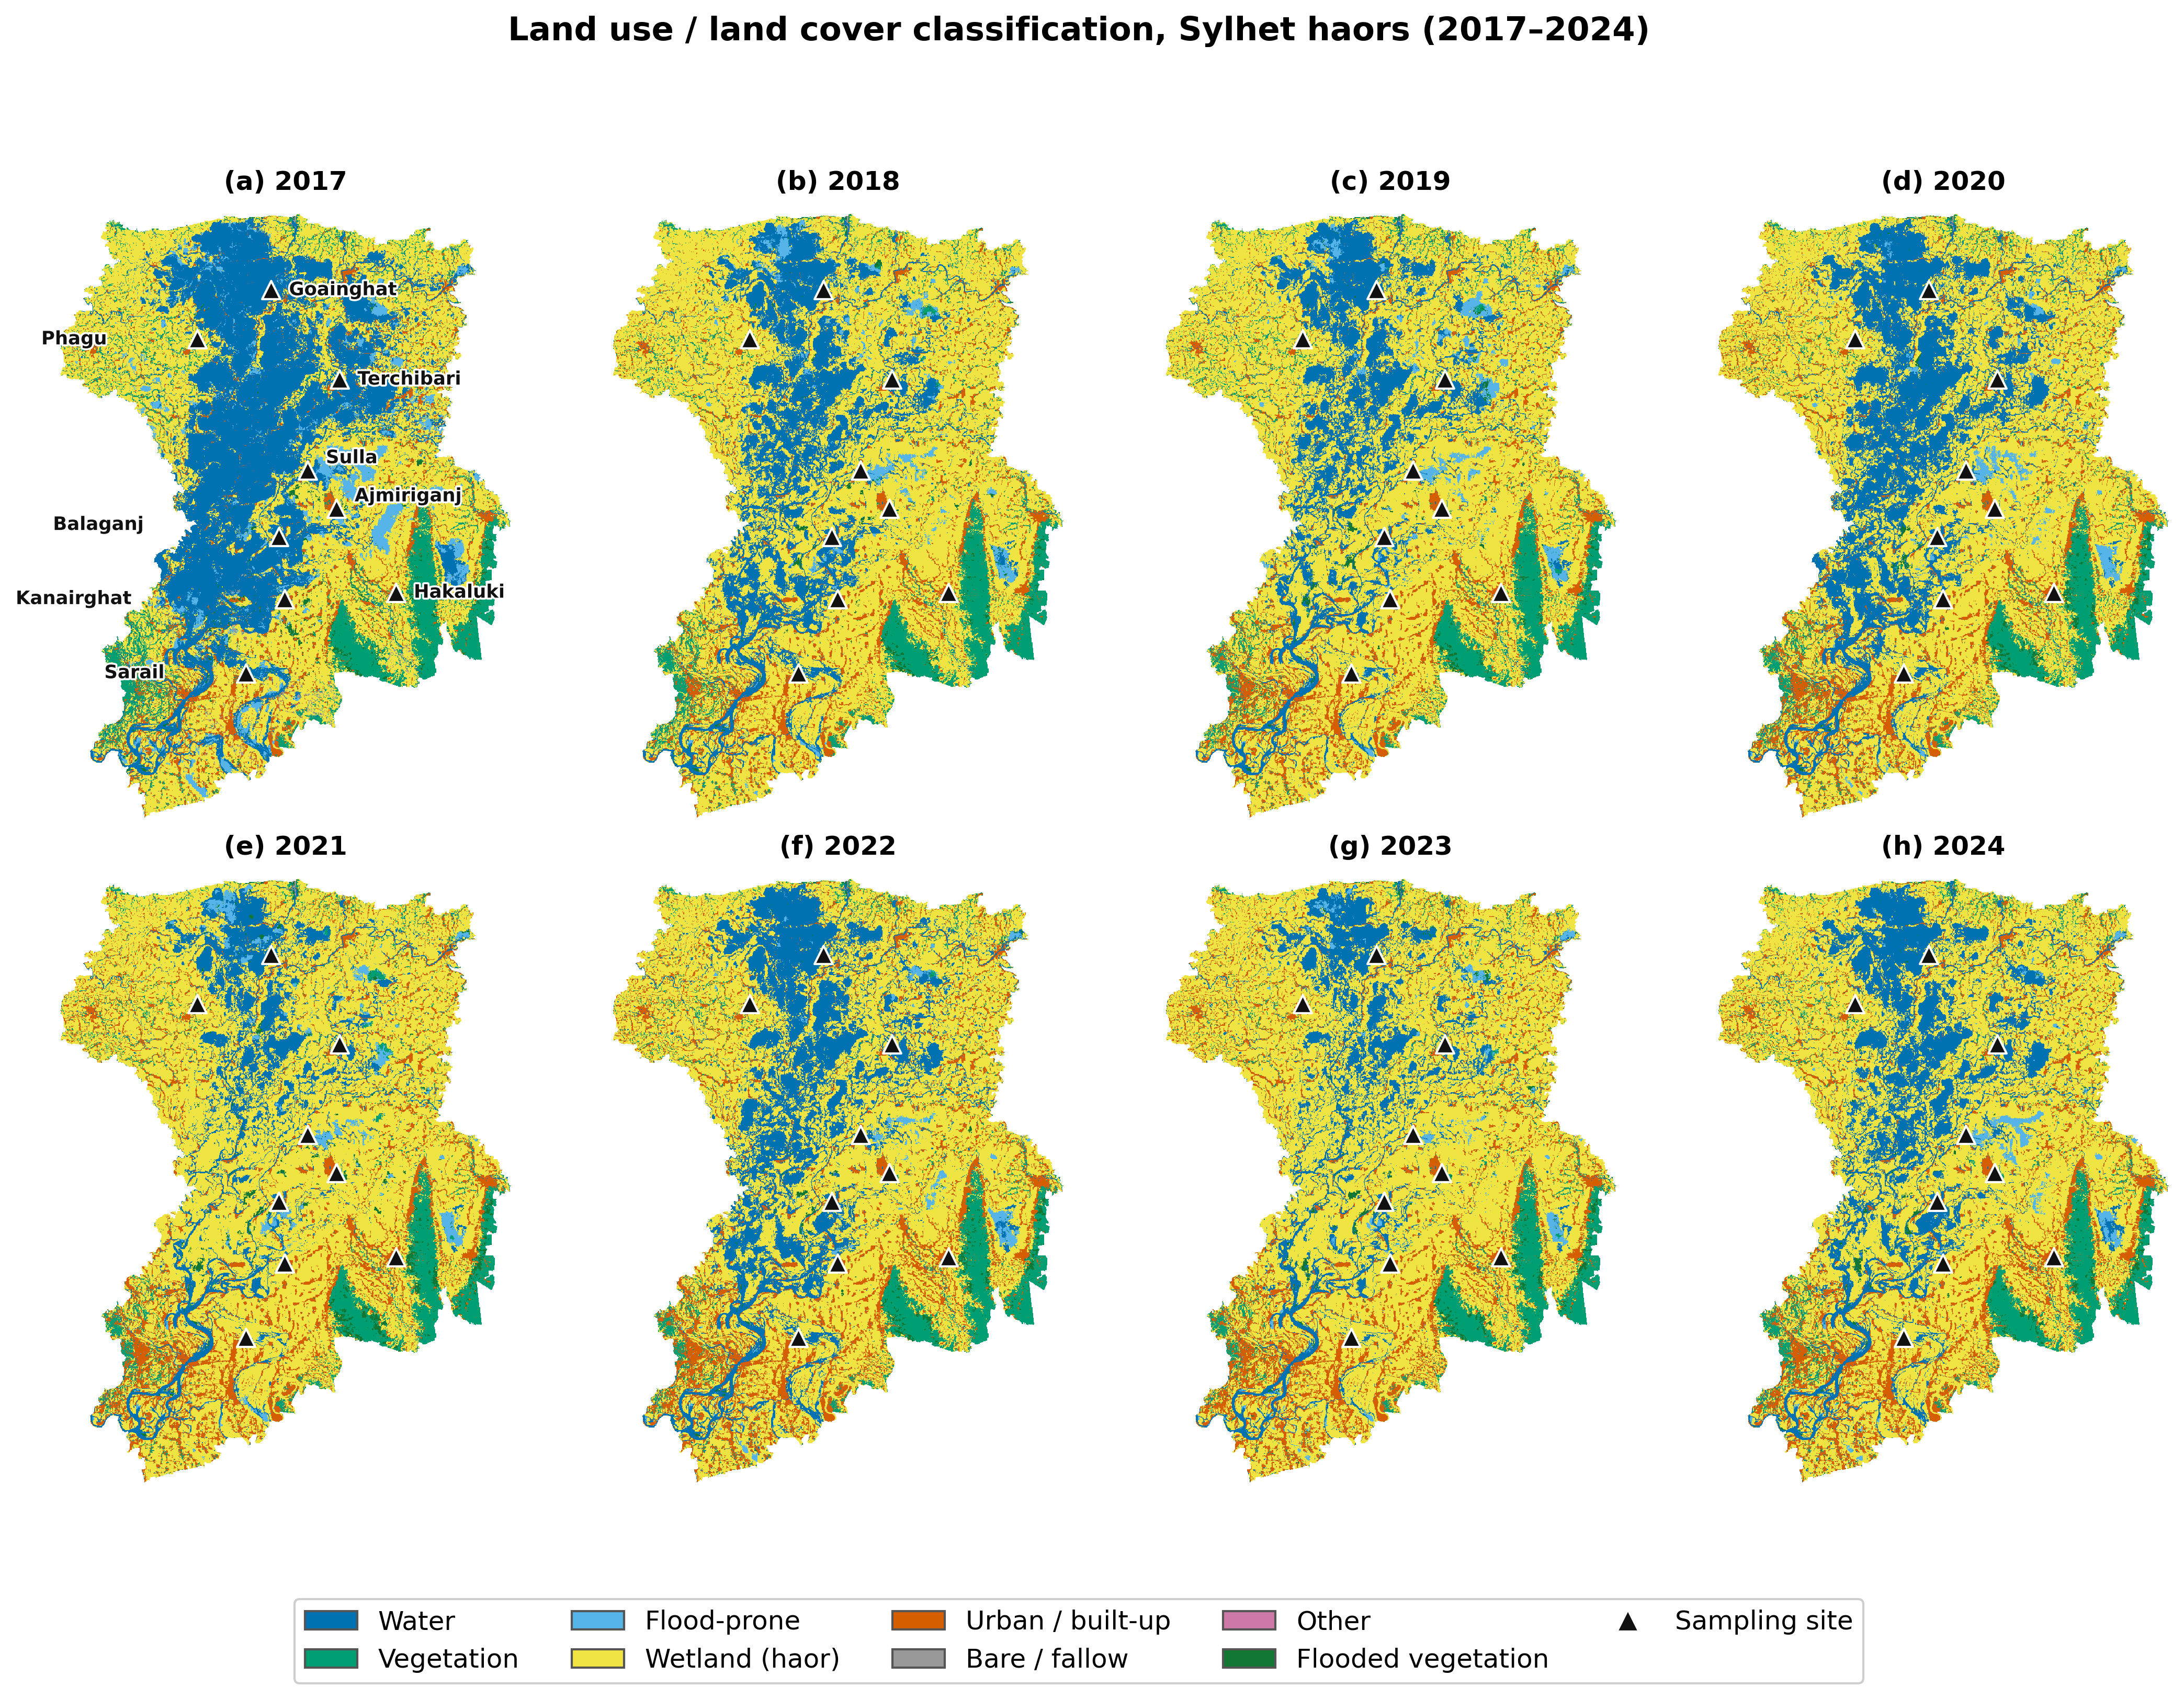
\includegraphics[width=0.8\textwidth]{Fig6_LULCMaps.png}
\caption{Sentinel-2 LULC classification of the Sylhet haors, 2017--2024 (annual maps),
with the nine sampling sites marked and labelled. The open-water class (blue) fluctuates
markedly between years as the seasonal flood line migrates, while the combined water$+$wetland
footprint stays nearly constant; built-up area (at the margins) increases over the series.}
\label{fig:lulc-maps}\end{figure}

\begin{figure}[htbp]\centering
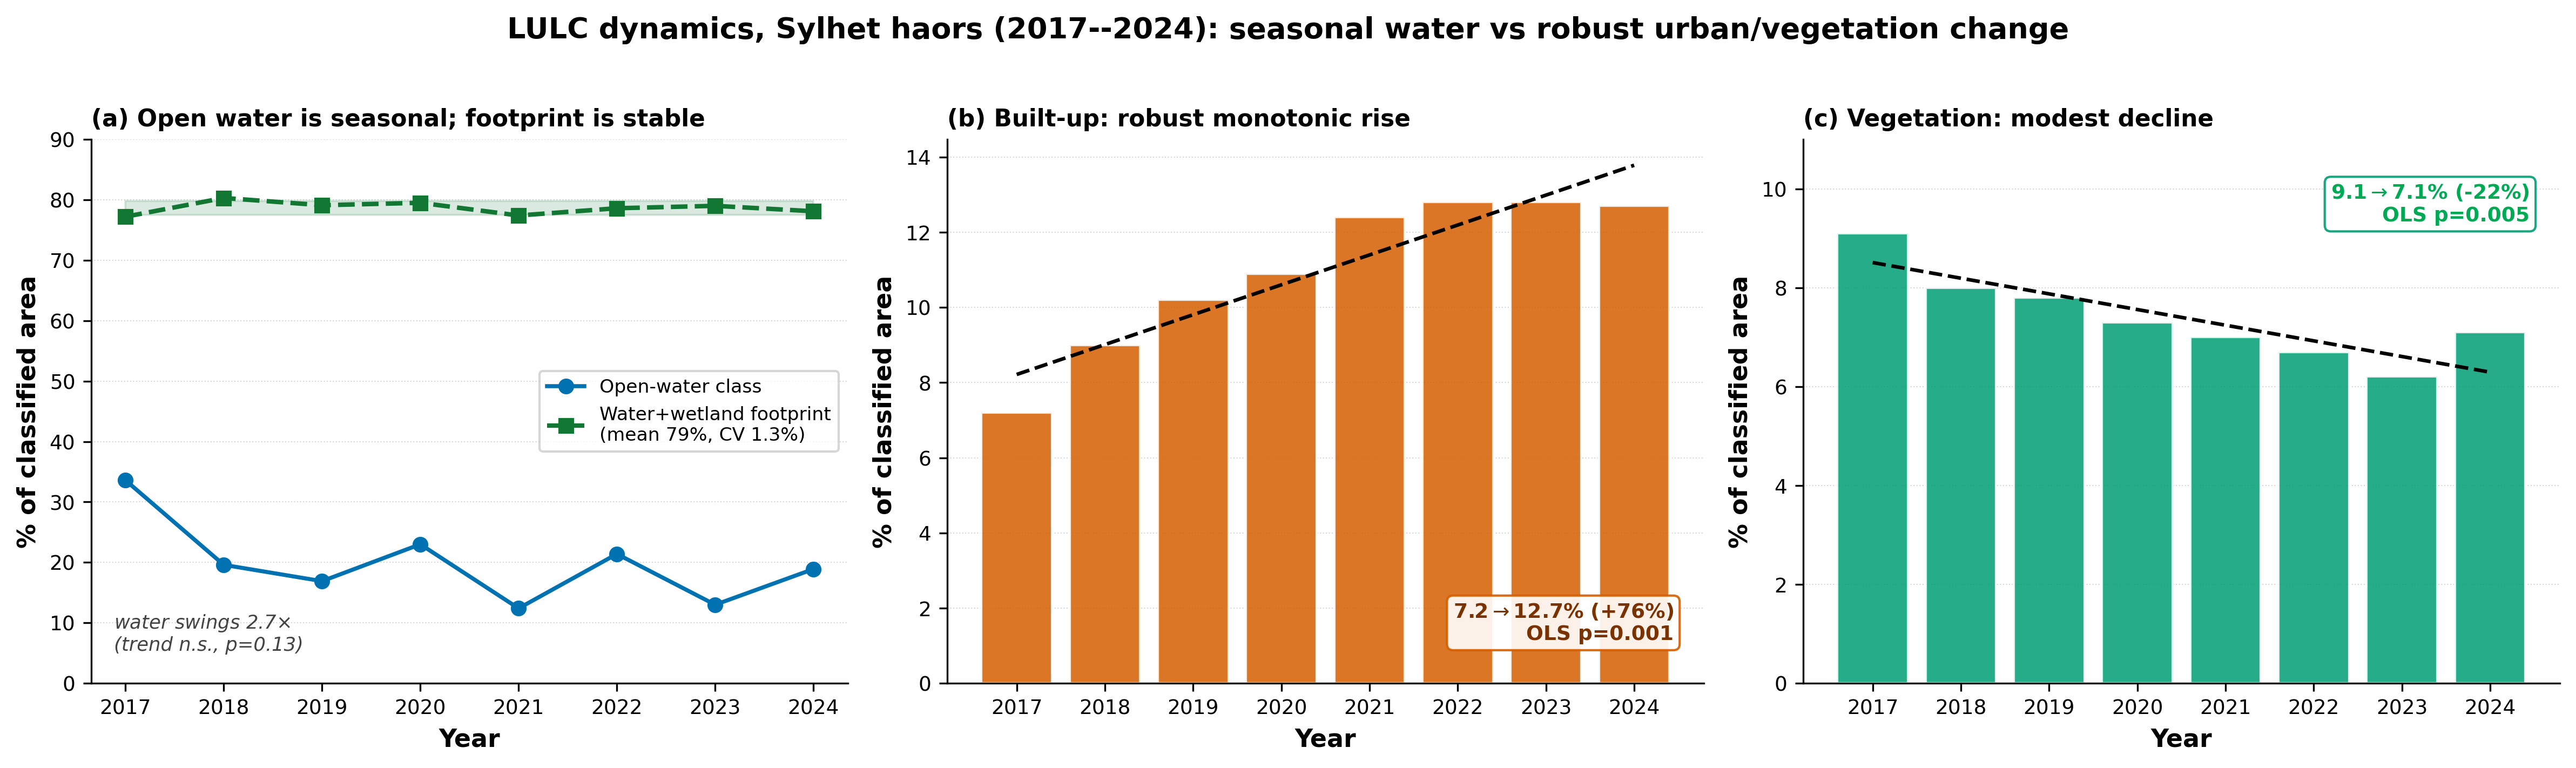
\includegraphics[width=0.75\textwidth]{Fig5_LULCChange.png}
\caption{LULC composition, 2017--2024 (\% of classified area). (a) The open-water class swings
2.7-fold between years while the combined water$+$wetland footprint stays nearly constant
(mean 79\%, CV 1.3\%), showing the swings are seasonal hydroperiod, not wetland loss;
(b) built-up area rises monotonically ($+$76\%); (c) the vegetation class declines modestly
($-$22\%).}
\label{fig:lulc-change}\end{figure}

\subsection{Site-scale LULC context and relation to SOC}
\label{subsec:local-lulc}
Within 500 m buffers (78.54 ha) around each site, the one consistent and seasonally robust
change was built-up expansion, which increased at almost every site, most strongly at
Hakaluki ($+$9.95~ha), Phagu ($+$8.87~ha) and Sulla ($+$7.70~ha) (Table~\ref{tab:buffer},
built-up column). The per-site water and flood-prone changes in Table~\ref{tab:buffer} are
reported for completeness but, as at the regional scale, are dominated by the seasonal
water$\leftrightarrow$exposed-bed exchange and should not be read as wetland conversion. Even
taken at face value, this recent site-scale change did not align with present SOCiT---sites with
the largest buffer-scale water or flooded-vegetation differences (e.g.\ Terchibari, Hakaluki)
did not have correspondingly low SOCiT---indicating that 2025 SOC reflects longer-term
management legacies rather than the most recent LULC dynamics, consistent with the
decadal-to-centennial timescales of soil-carbon turnover \citep{Trumbore1997}.

\begin{table}[htbp]\centering
\caption{Per-site land-cover area change within 500 m buffers, 2017--2024 (ha), recomputed
from the classified Sentinel-2 rasters. The built-up column is the seasonally robust signal;
water and flood-prone columns are largely seasonal (water$\leftrightarrow$exposed-bed exchange;
see Section~\ref{subsec:lulc-change}) and are not interpreted as wetland conversion.}
\label{tab:buffer}
\begin{tabular}{lrrrr}
\hline
Site & Water & Flood-prone & Flooded veg. & Built-up \\
\hline
Ajmiriganj & $0.0$ & $0.0$ & $+0.0$ & $+7.5$ \\
Balaganj & $-19.7$ & $-7.0$ & $0.0$ & $+3.8$ \\
Goainghat & $0.0$ & $0.0$ & $0.0$ & $0.0$ \\
Hakaluki & $0.0$ & $0.0$ & $-8.1$ & $+10.0$ \\
Kanairghat & $0.0$ & $-0.7$ & $-0.7$ & $+3.9$ \\
Phagu & $-1.5$ & $0.0$ & $0.0$ & $+8.9$ \\
Sarail & $-19.6$ & $0.0$ & $-0.4$ & $+1.1$ \\
Sulla & $+1.1$ & $0.0$ & $0.0$ & $+7.7$ \\
Terchibari & $-33.9$ & $-2.5$ & $+0.0$ & $-0.8$ \\
\hline
\end{tabular}
\end{table}

\subsection{Multi-decadal warming, drying, and greening (1988--2025)}
\label{subsec:indices}
Whole-year mean indices over these seasonally flooded haors are dominated by the open-water
fraction in each year's imagery (annual NDVI and NDWI correlate at $r=-0.89$), so we analyse
\emph{dry-season} (February--April) composites, in which standing water is minimal ($\sim$1.3\%
of the area, no temporal trend; Section~\ref{subsec:rs}). Two trends are then clear and robust
(Fig.~\ref{fig:env-indices}). First, dry-season NDVI \textbf{increased significantly}, from 0.47
in 1988 to 0.57 in 2025 (Mann--Kendall $p<0.001$; Sen's slope $+0.031$ decade$^{-1}$; a $+22$\%
greening), with the land-only NDVI essentially identical (Mann--Kendall $p<0.001$). This greening
reflects agricultural intensification---the expansion and densification of dry-season irrigated
Boro rice---and is corroborated by the gain in classified vegetation greenness independent of the
(seasonally confounded) vegetation-\emph{area} change. Second, dry-season land surface temperature
\textbf{warmed significantly}, at $+0.55\,^{\circ}$C decade$^{-1}$ (Mann--Kendall $p=0.015$; OLS
$p=0.009$), from $26.3$ to $27.6\,^{\circ}$C, $\approx$$2.1\,^{\circ}$C over the record (an annual
re-extraction gave a consistent $+0.66\,^{\circ}$C decade$^{-1}$).

The hydrological trend requires care, because the optical water index is unreliable here: in
dry-season composites NDWI mirrors NDVI ($r=-0.97$) and carries no independent hydrological
information, while the annual-mean NDWI ``decline'' reported in earlier drafts was an artifact of
the seasonal open-water fraction. We therefore assessed drying with an independent, physically
based source---ERA5-Land reanalysis \citep{MunozSabater2021}, which does not depend on optical
imagery (Fig.~\ref{fig:hydro}). Over 1985--2025 the basin shows a coherent drying signal:
root-zone (0--100~cm) soil moisture declined significantly (Mann--Kendall $p=0.021$;
$-0.033$~m$^3$\,m$^{-3}$ decade$^{-1}$, $\approx-6$\%), annual precipitation declined
(Mann--Kendall $p=0.017$; $-161$~mm decade$^{-1}$, $\approx-9$\%), and 2~m air temperature warmed
($p<0.001$; $+0.18\,^{\circ}$C decade$^{-1}$)---the last an independent confirmation of the
satellite LST warming. The same signal appears in a second land model with a partly independent
formulation: GLDAS-2.1 \citep{Rodell2004} over 2000--2025 shows a significant decline in root-zone
soil moisture (Mann--Kendall $p=0.014$) and a significant rise in evapotranspiration ($p<0.001$),
the latter consistent with warming-driven evaporative demand drawing down soil water. We note
ERA5-Land and GLDAS are not fully independent---both ingest overlapping meteorological forcing---so
their agreement reflects consistency more than full corroboration. A genuinely independent
constraint comes from GRACE/GRACE-FO satellite gravimetry \citep{Tapley2004}, whose terrestrial
water storage trended downward over its shorter record (2003--2016), though not significantly
($p=0.66$). Taken together---two land models agreeing on declining soil moisture and rising
evaporative demand, falling rainfall, rising temperature, and a (weak) gravimetric decline---the
evidence consistently points to a drying basin, while acknowledging the products are
model-dependent. The haor is thus becoming both warmer and drier even though its inundated
\emph{footprint} (a seasonal, image-timing quantity) appears stable
(Section~\ref{subsec:lulc-change})---declining water content and rainfall need not shrink the
wet-season extent. These warming and drying trends together \textbf{support H1}, alongside the
agricultural intensification indicated by the greening. (The Built-Up Index showed no significant
trend, $p=0.30$; urbanization is quantified directly by the LULC built-up class,
Section~\ref{subsec:lulc-change}. The previously reported ``$+4\,^{\circ}$C'' warming and
``$+180\%$'' BUI rise were data artifacts and are not supported.) We note these soil-moisture and
monsoon-precipitation trends are model-based and should be read as converging reanalysis evidence
rather than ground truth.

\begin{figure}[htbp]\centering
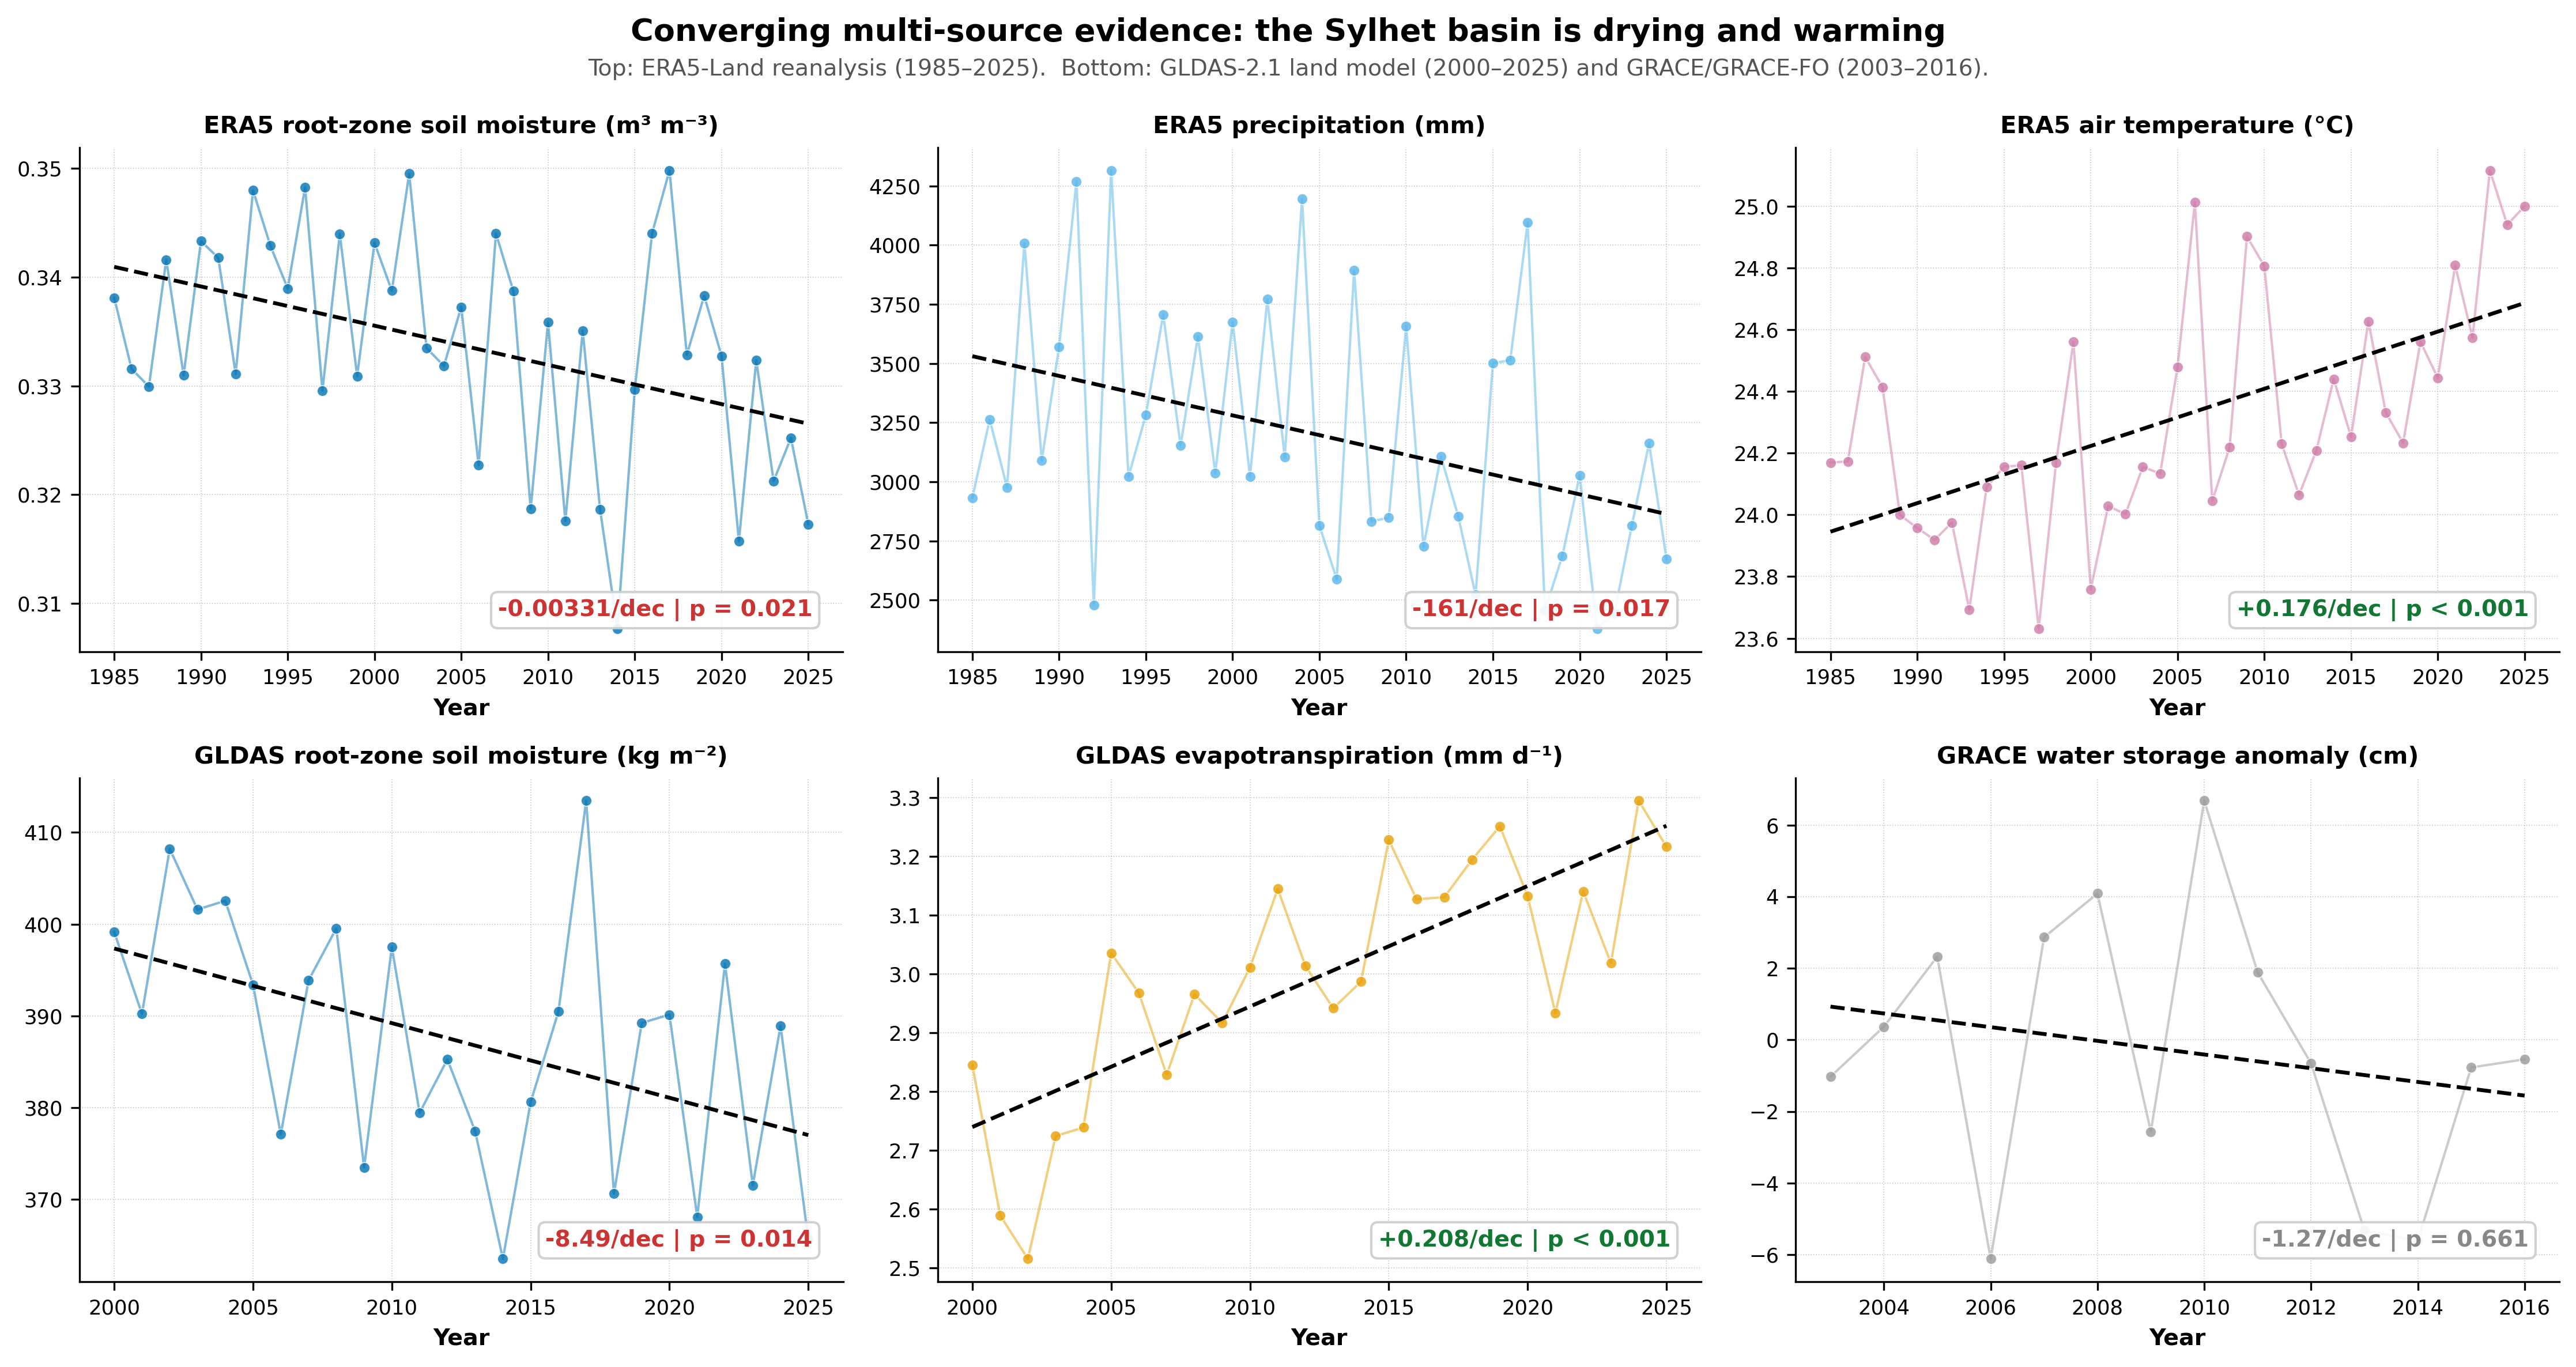
\includegraphics[width=0.95\textwidth]{Fig14_hydrology.png}
\caption{Converging multi-source basin hydrology, free of the optical water-fraction confound.
Top: ERA5-Land reanalysis (1985--2025)---root-zone soil moisture and precipitation decline
significantly while air temperature rises. Bottom: independent GLDAS-2.1 (2000--2025) confirms
declining root-zone soil moisture and rising evapotranspiration, and GRACE/GRACE-FO water storage
(2003--2016) trends downward (non-significant). Mann--Kendall statistics shown.}
\label{fig:hydro}\end{figure}

\begin{figure}[htbp]\centering
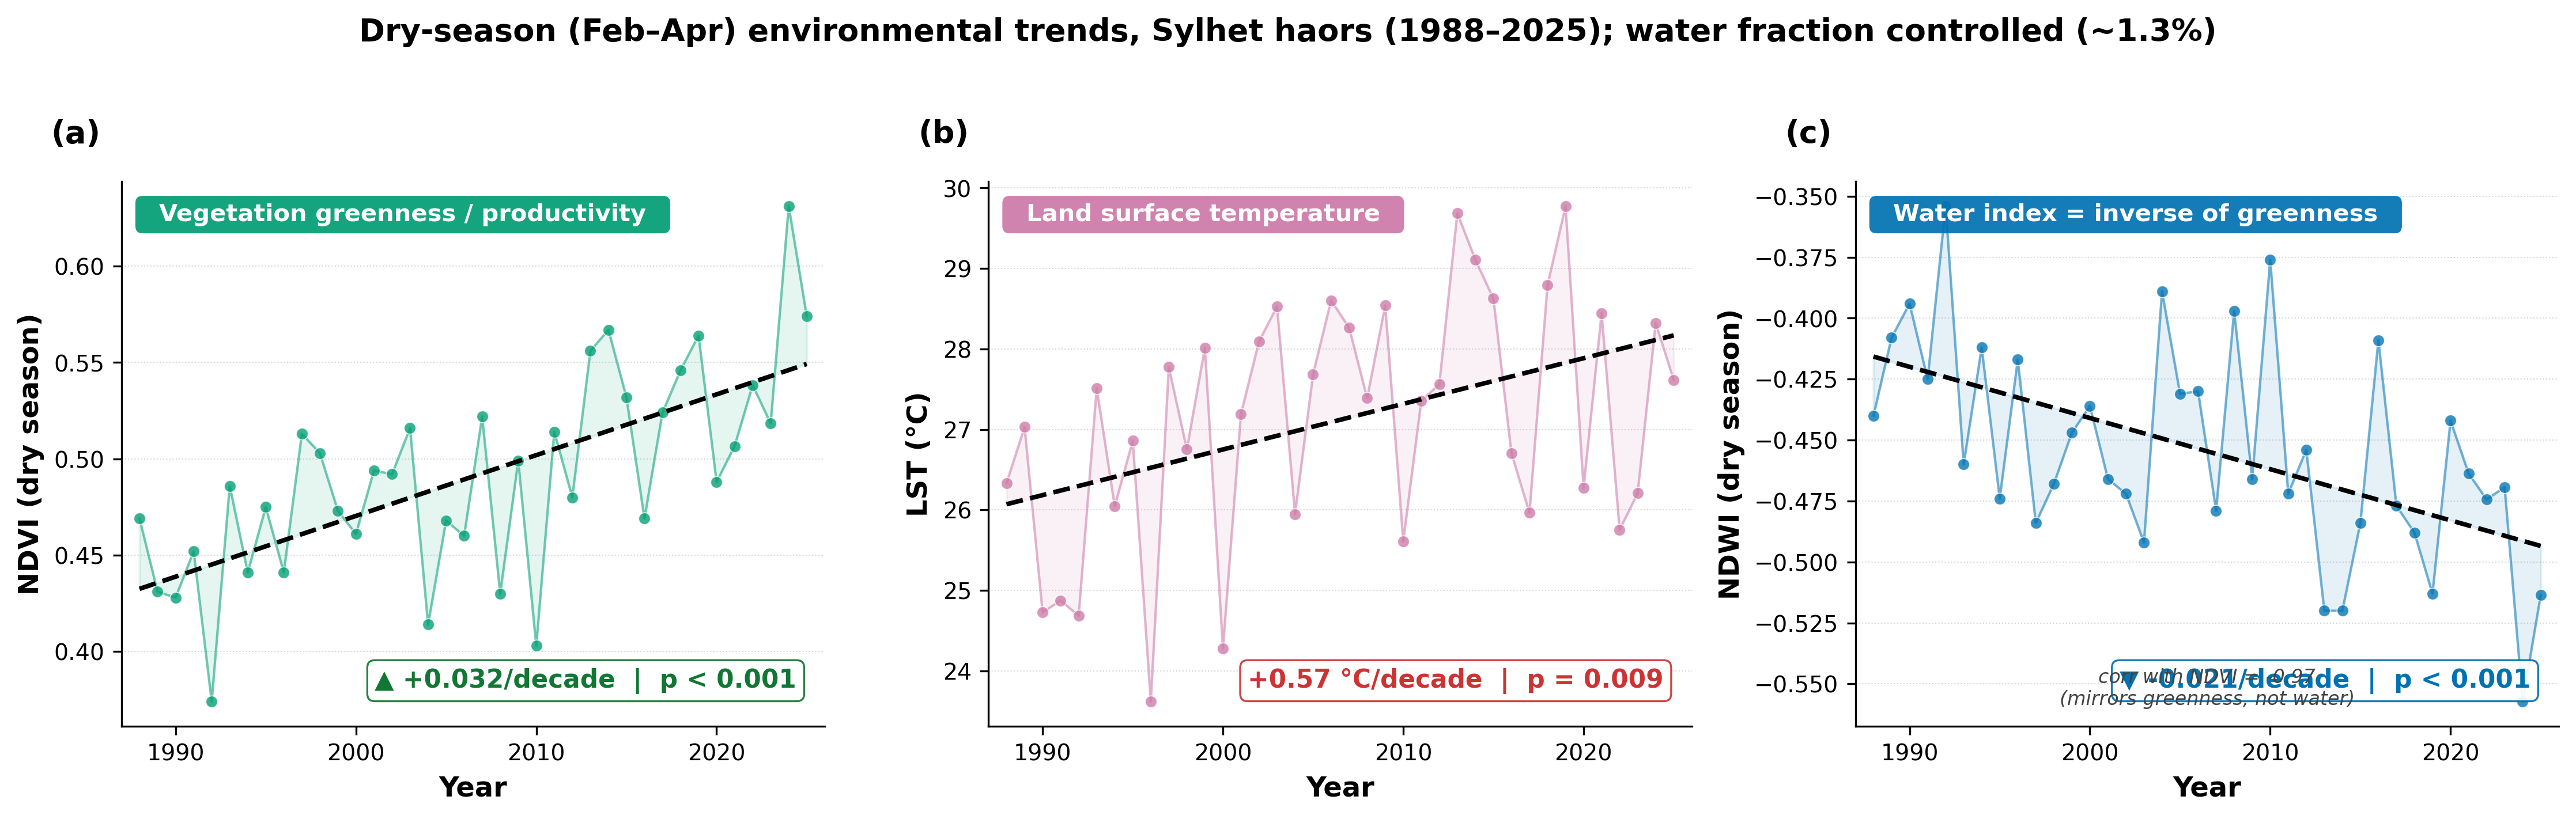
\includegraphics[width=0.95\textwidth]{Fig7_EnvIndices.png}
\caption{Dry-season (February--April), water-fraction-controlled environmental trends,
1988--2025: (a) NDVI greening, (b) LST warming, (c) NDWI, which mirrors NDVI ($r=-0.97$) and
is not an independent hydrological signal. Trend lines and statistics shown.}
\label{fig:env-indices}\end{figure}

\begin{figure}[htbp]\centering
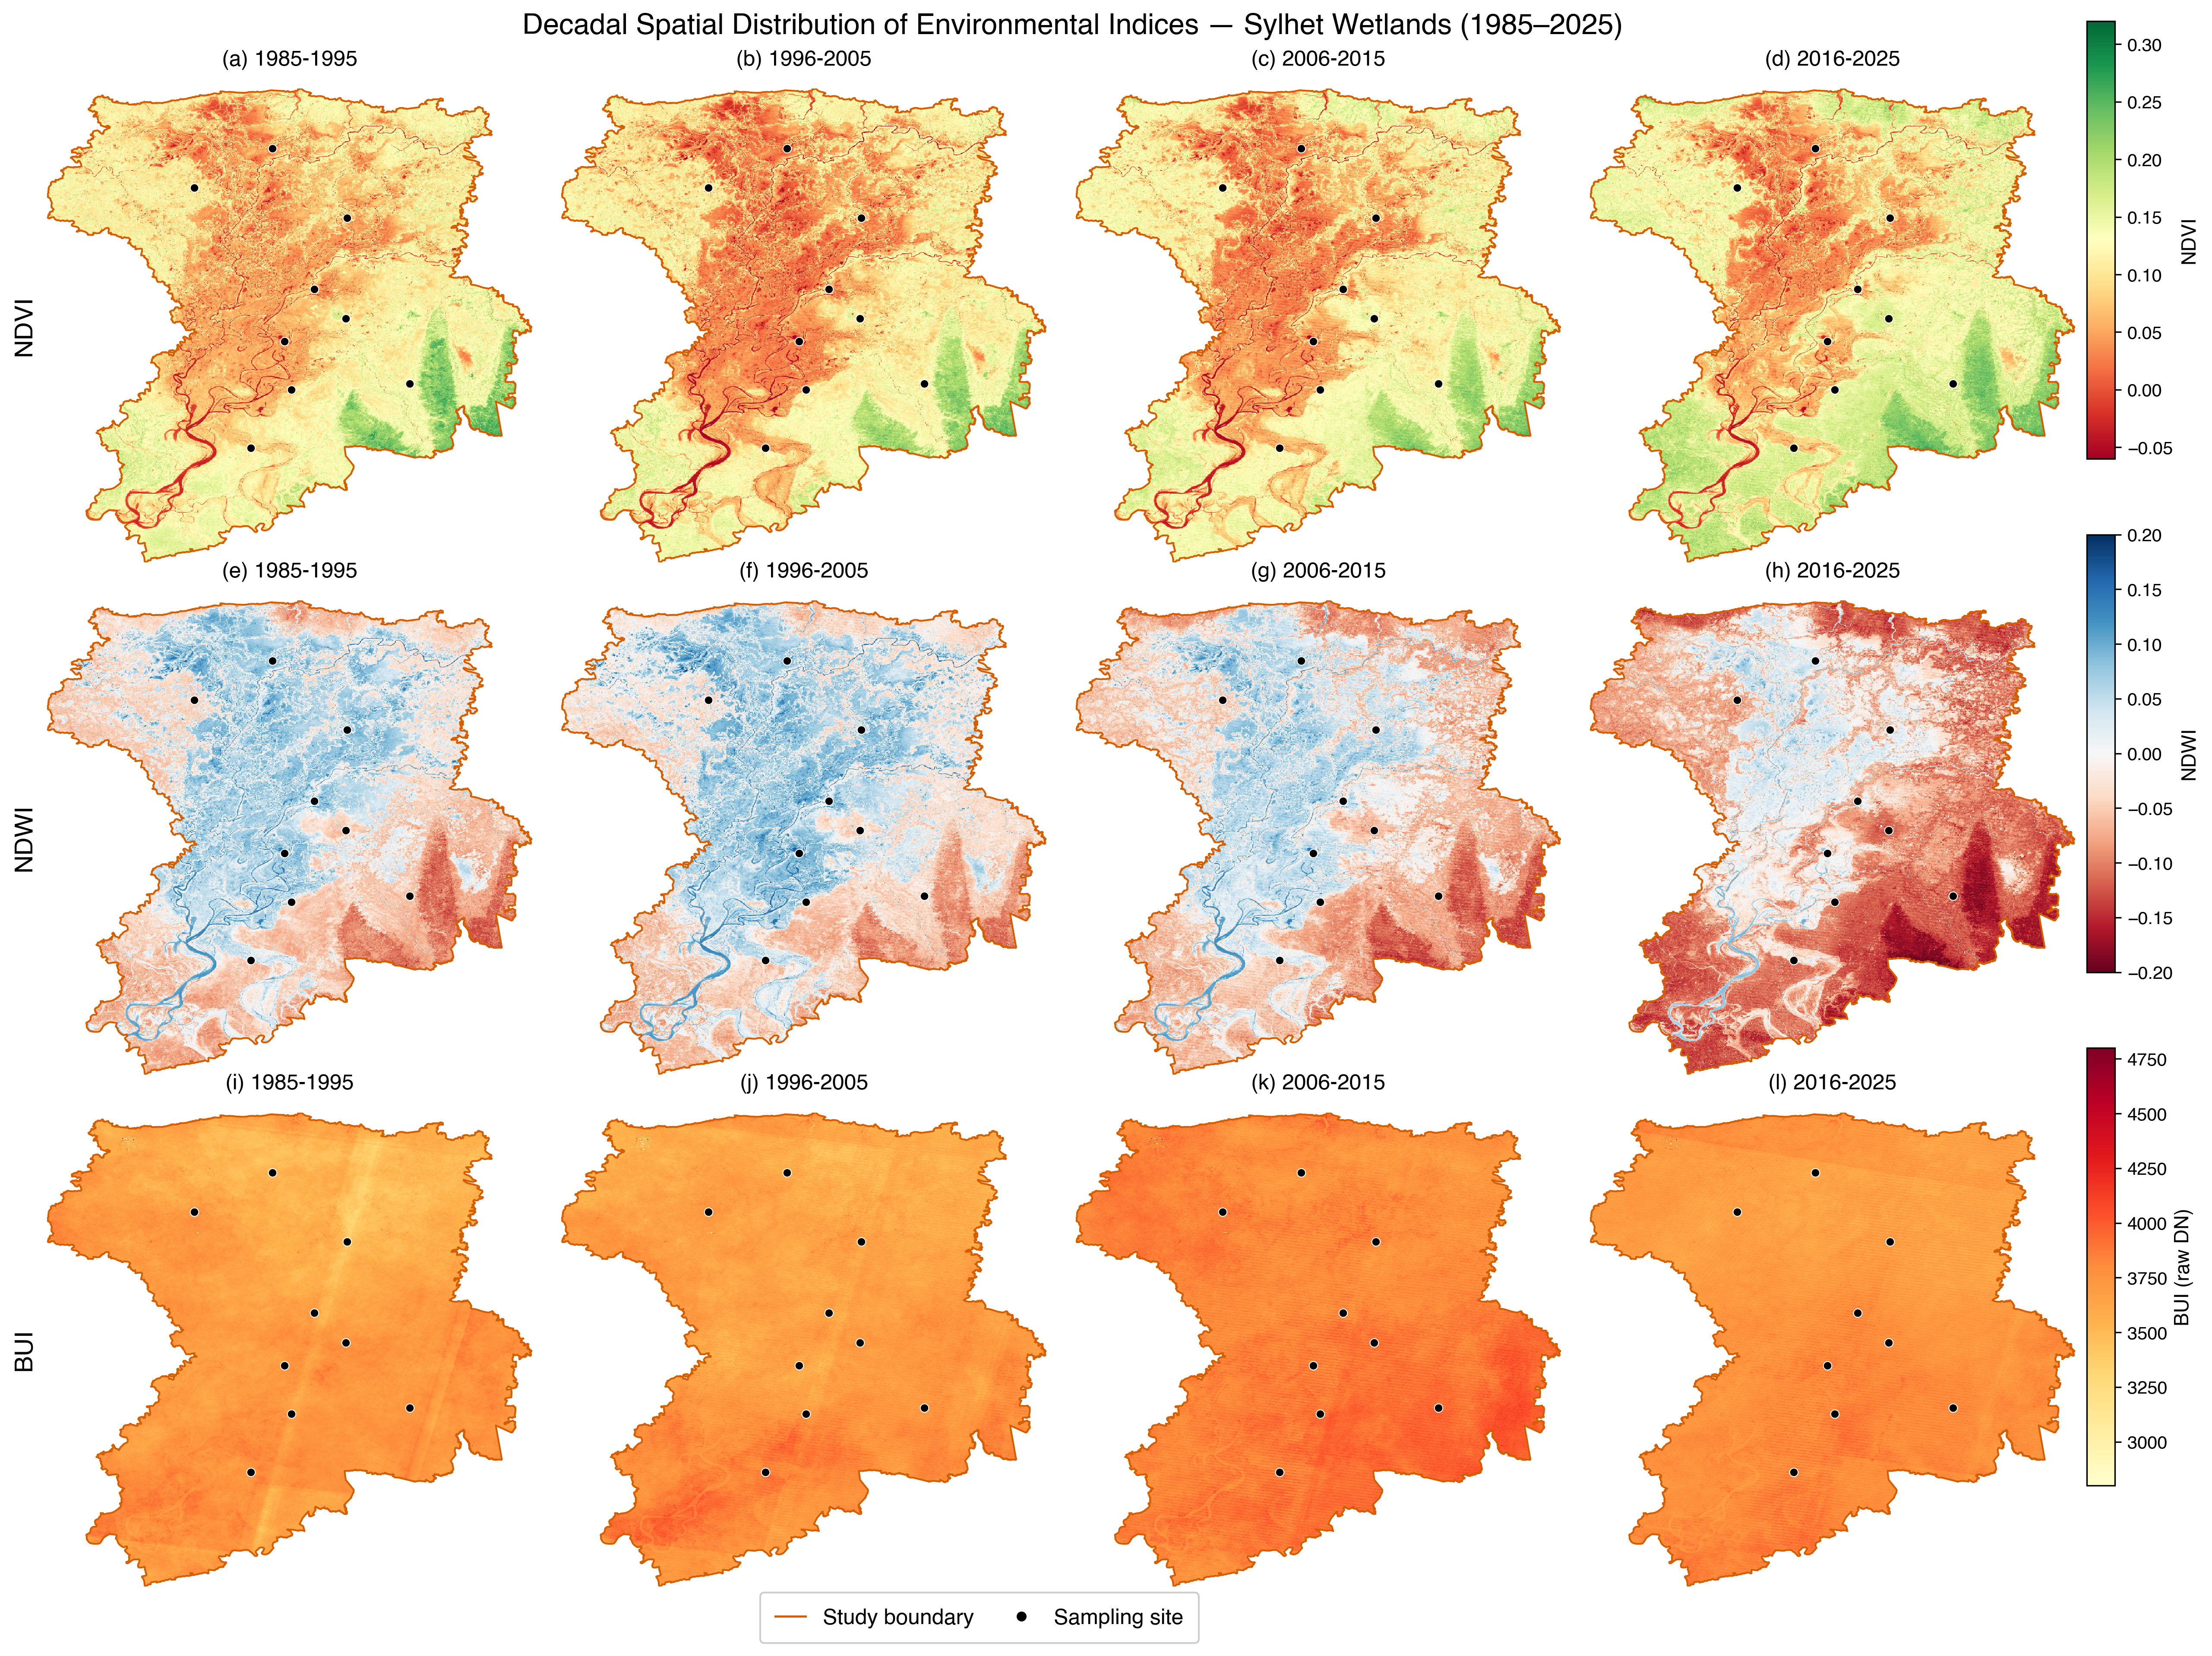
\includegraphics[width=0.75\textwidth]{Fig11_DecadalIndices.png}
\caption{Decadal spatial patterns of NDVI and NDWI across the basin, 1988--2025.}
\label{fig:decadal-indices}\end{figure}

\subsection{Vegetation biomass}
\label{subsec:biomass-results}
Applying Eq.~\ref{eq:biomass} to the dry-season NDVI series, estimated above-ground biomass
rose from $\approx$1.0 t ha$^{-1}$ yr$^{-1}$ in 1988 to $\approx$1.7 t ha$^{-1}$ yr$^{-1}$ in
2025 (range 0.5--2.2; OLS $p<0.001$, $r=0.67$; Fig.~\ref{fig:biomass}), tracking the greening
trend and consistent with intensifying dry-season cultivation. (We use dry-season NDVI here
because annual-mean NDVI for these flooded haors, 0.05--0.16, falls below the calibration range
of Eq.~\ref{eq:biomass} and on the descending limb of its quadratic, which would invert the
relationship; dry-season NDVI, 0.47--0.63, lies on the physically sensible ascending limb.)
Absolute values carry the transferability caveat noted in Section~\ref{subsec:biomass}; the
\emph{trend} is the interpretable result. ESA CCI standing AGB over 2010--2021 was
20.8--30.4 Mg ha$^{-1}$ (a complementary multi-year standing-stock measure) and broadly tracks
the NDVI record, though its short, gappy coverage means the Landsat series remains the basis for
multi-decadal inference.

\begin{figure}[htbp]\centering
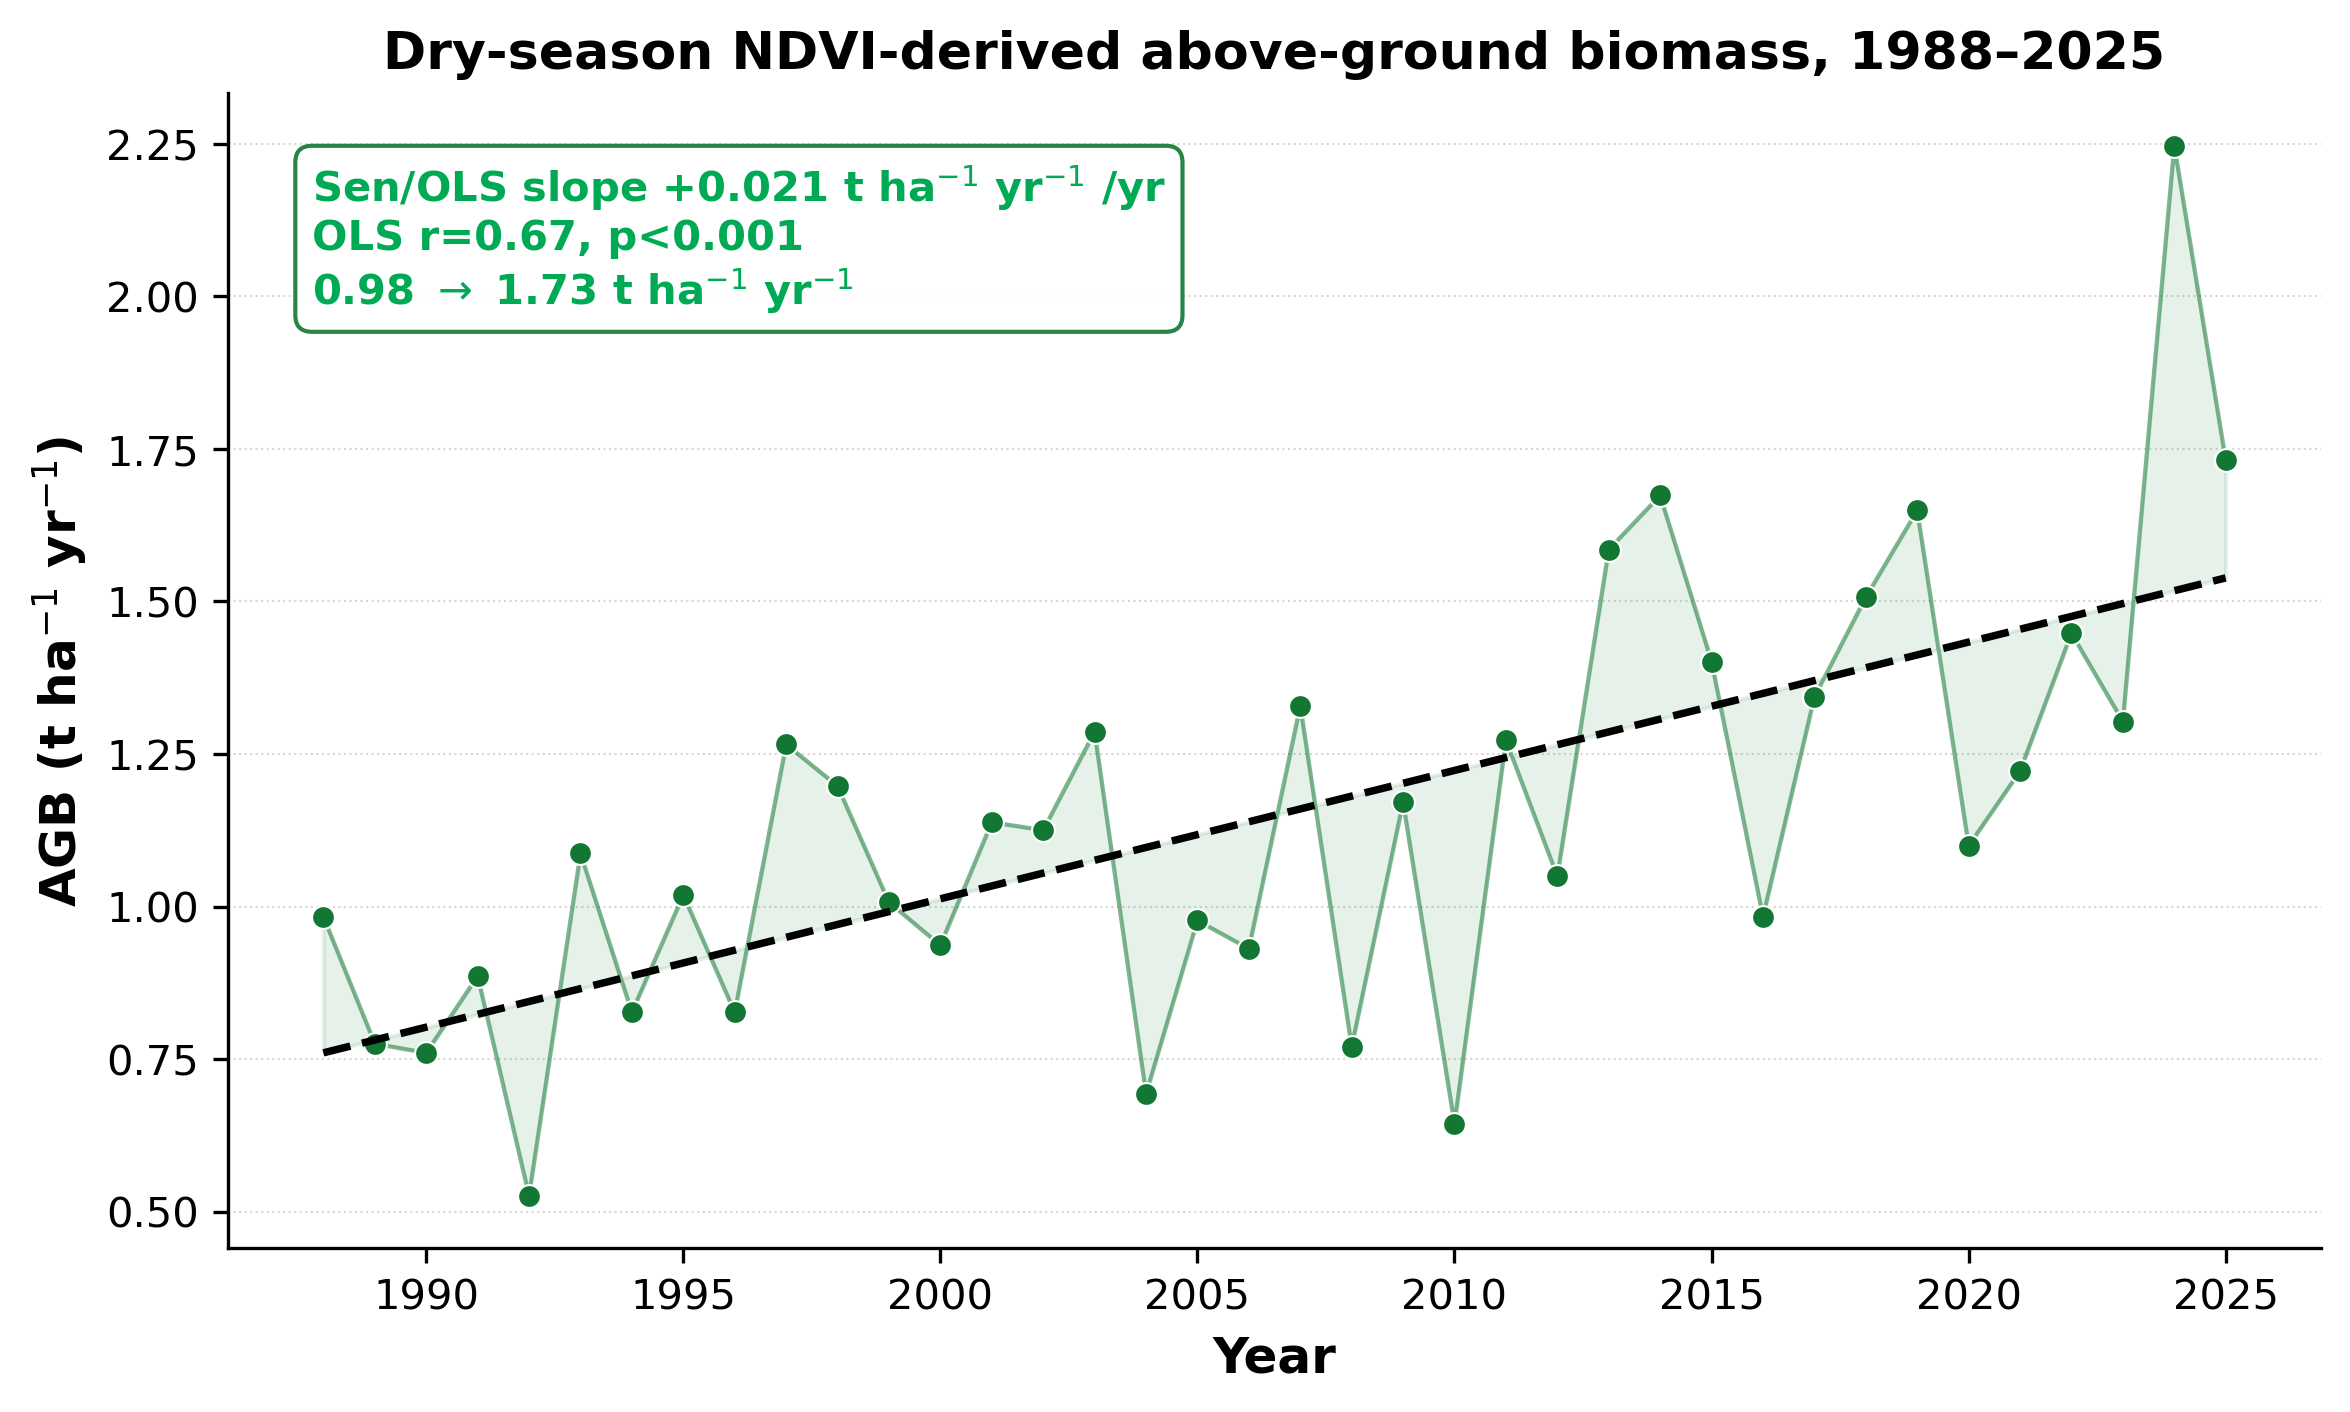
\includegraphics[width=0.7\textwidth]{Fig8_VegBiomass.png}
\caption{Dry-season NDVI-derived above-ground biomass, 1988--2025, increasing with the
greening trend ($+$0.021 t ha$^{-1}$ yr$^{-1}$ per year, $p<0.001$).}
\label{fig:biomass}\end{figure}

\subsection{Exploratory multivariate structure (PCA)}
\label{subsec:pca}
% Reviewer comment 36 -- loadings table, corrected interpretation.
A PCA of standardized 2025 soil variables ($n=9$; exploratory) is summarized in
Table~\ref{tab:pca} and Fig.~\ref{fig:pca-clustering}. The first two components explained
87.4\% of variance (PC1 52.9\%, PC2 34.5\%). PC1 was defined by clay, CEC and pH (the
texture--exchange complex); \emph{SOC and TN loaded together on PC2, separately from clay}.
This multivariate structure reinforces the bivariate result: SOC aligns with nitrogen/OM, not
with soil texture---again contrary to H2. Hierarchical clustering and DBSCAN (exploratory)
broadly recovered the same texture--exchange vs.\ organic-matter axes; we do not over-interpret
cluster membership given $n=9$.

\begin{table}[htbp]\centering
\caption{PCA of standardized 2025 soil variables ($n=9$): eigenvalues, variance explained,
and loadings (PC1--PC3).}
\label{tab:pca}
\begin{tabular}{lrrr}
\hline
 & PC1 & PC2 & PC3 \\
\hline
Eigenvalue & 3.57 & 2.33 & 0.52 \\
\% variance & 52.9 & 34.5 & 7.7 \\
Cumulative \% & 52.9 & 87.4 & 95.1 \\
\hline
SOC\% & $-0.18$ & $+0.62$ & $+0.06$ \\
Clay  & $+0.51$ & $+0.24$ & $+0.26$ \\
pH    & $+0.48$ & $-0.25$ & $+0.44$ \\
CEC   & $+0.53$ & $+0.17$ & $+0.08$ \\
TN    & $-0.17$ & $+0.62$ & $+0.36$ \\
SBD   & $-0.41$ & $-0.30$ & $+0.77$ \\
\hline
\end{tabular}
\end{table}

\begin{figure}[htbp]\centering
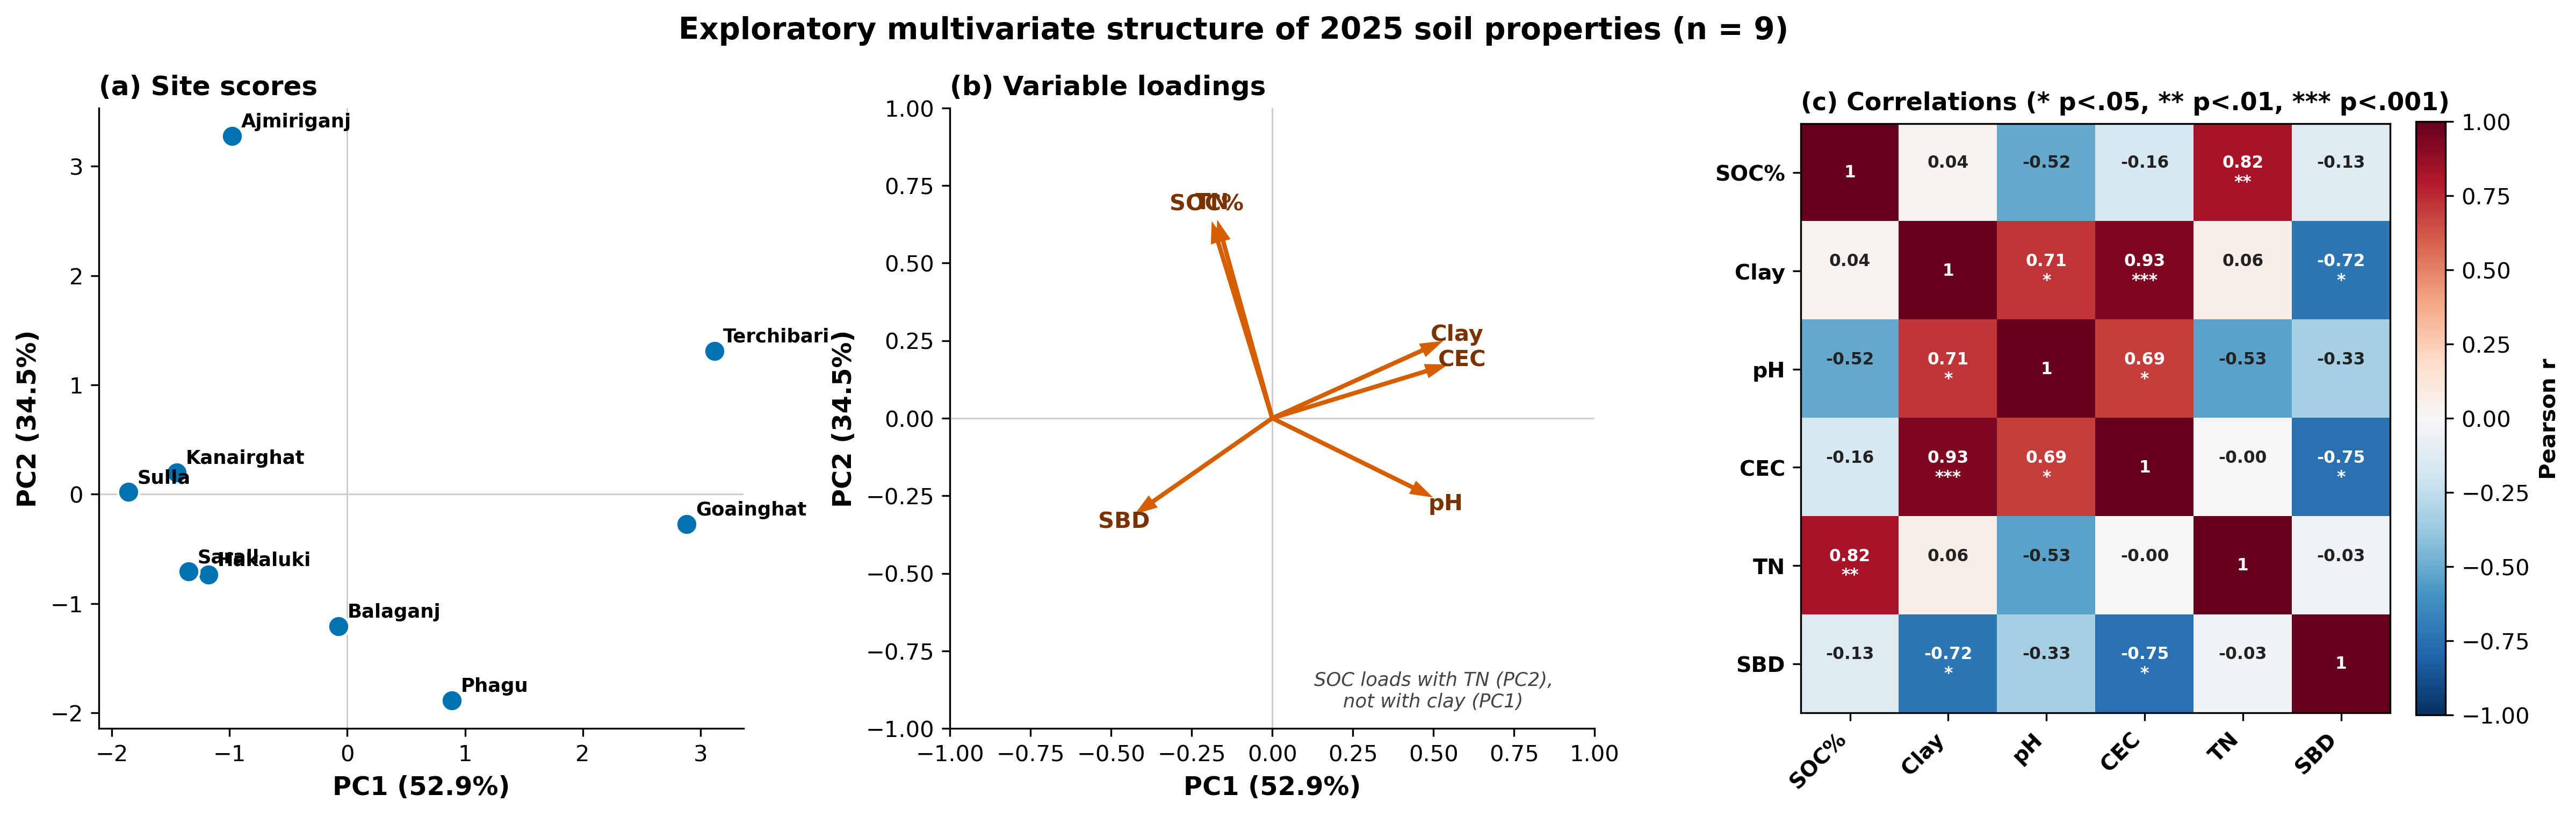
\includegraphics[width=0.75\textwidth]{Fig9_SOC_PCA_Corr.png}
\caption{PCA biplot and correlation matrix of 2025 soil variables. [Fig to be redrawn:
separate score and loading plots; remove redundant axis legend; add significance markers to
the correlation matrix---reviewer comments 35, 37.]}
\label{fig:pca-clustering}\end{figure}

\subsection{External benchmarking against comparable soils (WoSIS)}
\label{subsec:wosis}
Because our inferences rest on nine sites, we tested whether the observed SOC--property
relations hold in the wider population of comparable soils, using the WoSIS global profile
database \citep{Batjes2020} restricted to the Sylhet soil class (acidic, clay-rich;
Section~\ref{subsec:stats}). The result reproduces our site-level pattern at scale
(Fig.~\ref{fig:wosis}). Within this class ($n=9{,}676$ global profiles), topsoil SOC was
only weakly related to clay ($\rho=+0.12$), and this clay--SOC association \emph{disappeared}
when organic-matter content (indexed by total nitrogen) was held constant (partial $\rho=+0.01$),
indicating that clay carries essentially no information about SOC beyond that already conveyed by
organic-matter quantity. (SOC and total N co-vary strongly, $\rho=+0.81$, but as noted in
Section~\ref{subsec:soc-2025} this partly reflects the constrained C:N of soil organic matter, so
we use N only as a proxy for organic-matter quantity, not as an independent control.) The same
held in genuine land-cover subsets of the class: in cultivated/paddy soils
($n=2{,}425$)---the closest analogue to the haor Boro-rice setting---clay--SOC was $\rho=+0.07$
with a partial $\rho=+0.02$, and in herbaceous-wetland soils ($n=96$) $\rho=+0.29$
falling to a partial $\rho=+0.06$ (Fig.~\ref{fig:wosis}a). For reference, across \emph{all} soils clay shows a modest positive
association with SOC ($\rho=+0.25$ globally), so the texture decoupling is a property of this
already clay-rich, acidic regime rather than a universal rule. Finally, the Sylhet sites fall
near---and somewhat below---the median of cultivated soils of their class (Fig.~\ref{fig:wosis}b;
$\sim$31st percentile, $n=2{,}425$): they hold typical-to-moderate SOC for paddy soils of this
type, richer than regional uplands but not exceptional within their own class. This benchmarking
turns a nine-site observation into a generalizable result: in clay-rich, acidic wetland soils,
SOC is set by organic-matter and nitrogen supply, not by mineral (clay) protection capacity.

The same dataset also lets us test, by space-for-time substitution, whether warming plausibly
depresses SOC. Joining WorldClim \citep{Hijmans2005} mean annual temperature (MAT) and
precipitation (MAP) to the soil class, SOC declined with temperature, but the apparent strength
of that effect depends critically on the breadth of the climate gradient. Across the full class
(MAT $-12$ to $+30\,^{\circ}$C), temperature was the strongest predictor in a standardized
log-SOC regression ($\beta_{\mathrm{MAT}}=-0.38$; Fig.~\ref{fig:climate}); however, much of this
reflects climate-zone differences in decomposition rather than a within-climate effect. When we
restrict to climates comparable to Sylhet---warm, wet conditions (MAT 20--30\,$^{\circ}$C, MAP
$>$1200~mm; $n=2{,}947$)---the temperature effect shrinks but remains negative
($\beta_{\mathrm{MAT}}=-0.11$; partial $\rho_{\mathrm{MAT\cdot N,MAP}}=-0.12$), while
organic-matter quantity (indexed by total nitrogen) becomes the dominant correlate
($\beta_{\mathrm N}=+0.47$). The same holds across monsoon-Asian cultivated soils, the closest
haor analogue. We therefore report a deliberately conservative conclusion: within Sylhet-like
climates, warmer conditions are associated with modestly lower SOC after accounting for nitrogen
and rainfall, but organic-matter quantity is the primary correlate---consistent with the field
result. Two caveats apply: this is a
spatial substitution for time, and even the climate-restricted estimate is observational. With
these caveats, the analysis indicates the basin's $+0.55\,^{\circ}$C decade$^{-1}$ warming is a
plausible secondary pressure on these carbon stores, operating on top of the dominant
management/organic-matter control.

\begin{figure}[htbp]\centering
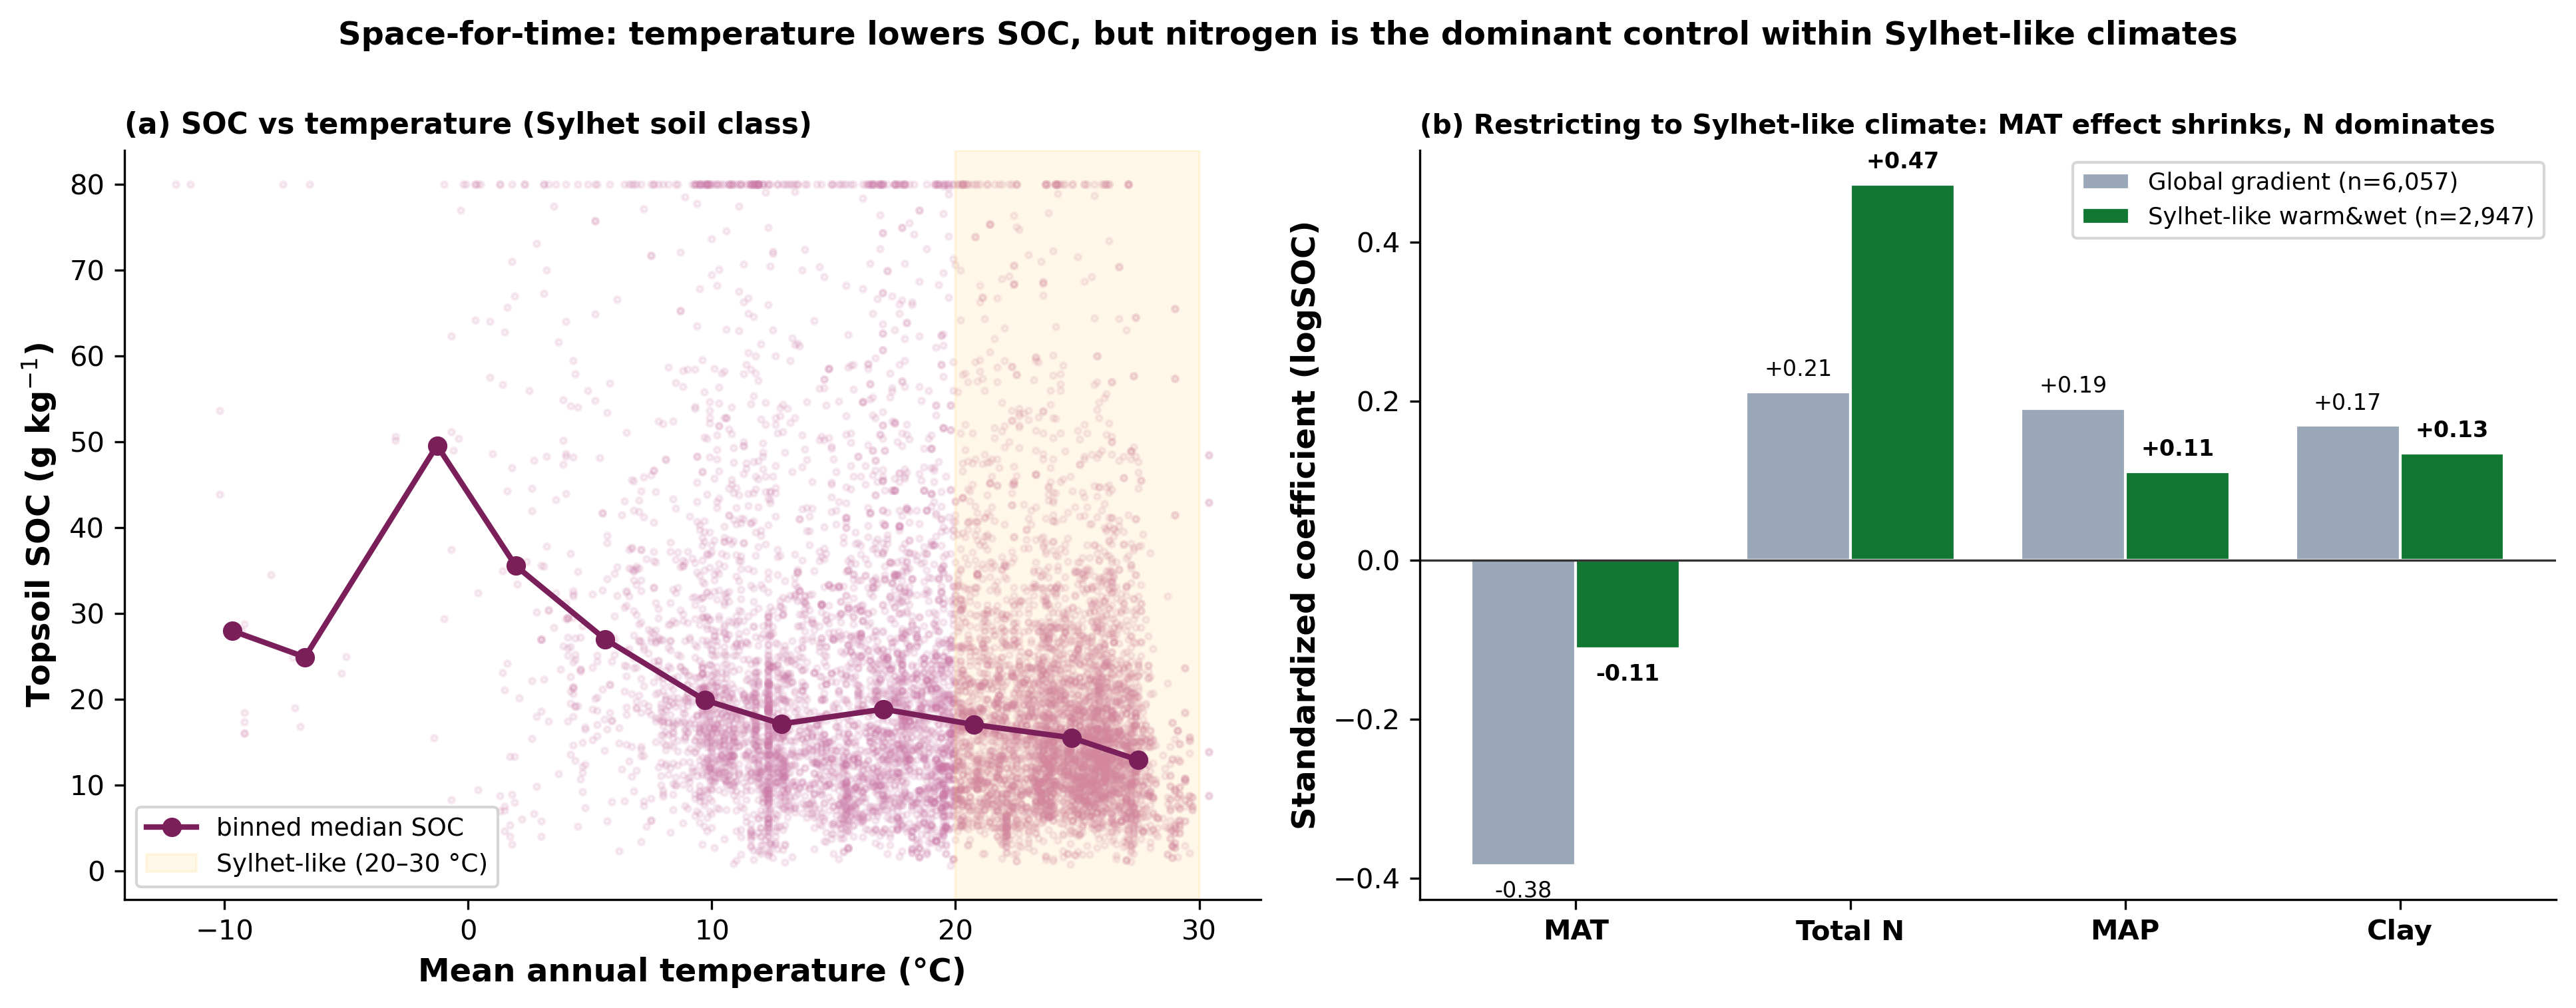
\includegraphics[width=0.95\textwidth]{Fig13_climate_soc.png}
\caption{Space-for-time test within the Sylhet soil class (WoSIS $+$ WorldClim). (a) Topsoil SOC
versus mean annual temperature (points; line is binned median); the shaded band marks Sylhet-like
warm conditions. (b) Standardized log-SOC regression coefficients for the full global gradient
versus the Sylhet-like warm-and-wet restriction (MAT 20--30\,$^{\circ}$C, MAP $>$1200~mm,
$n=2{,}947$): restricting to the local climate shrinks the temperature effect
($\beta_{\mathrm{MAT}}$: $-0.38\rightarrow-0.11$) and leaves nitrogen as the dominant control
($\beta_{\mathrm N}=+0.47$), removing the global climate-zone confound.}
\label{fig:climate}\end{figure}

\begin{figure}[htbp]\centering
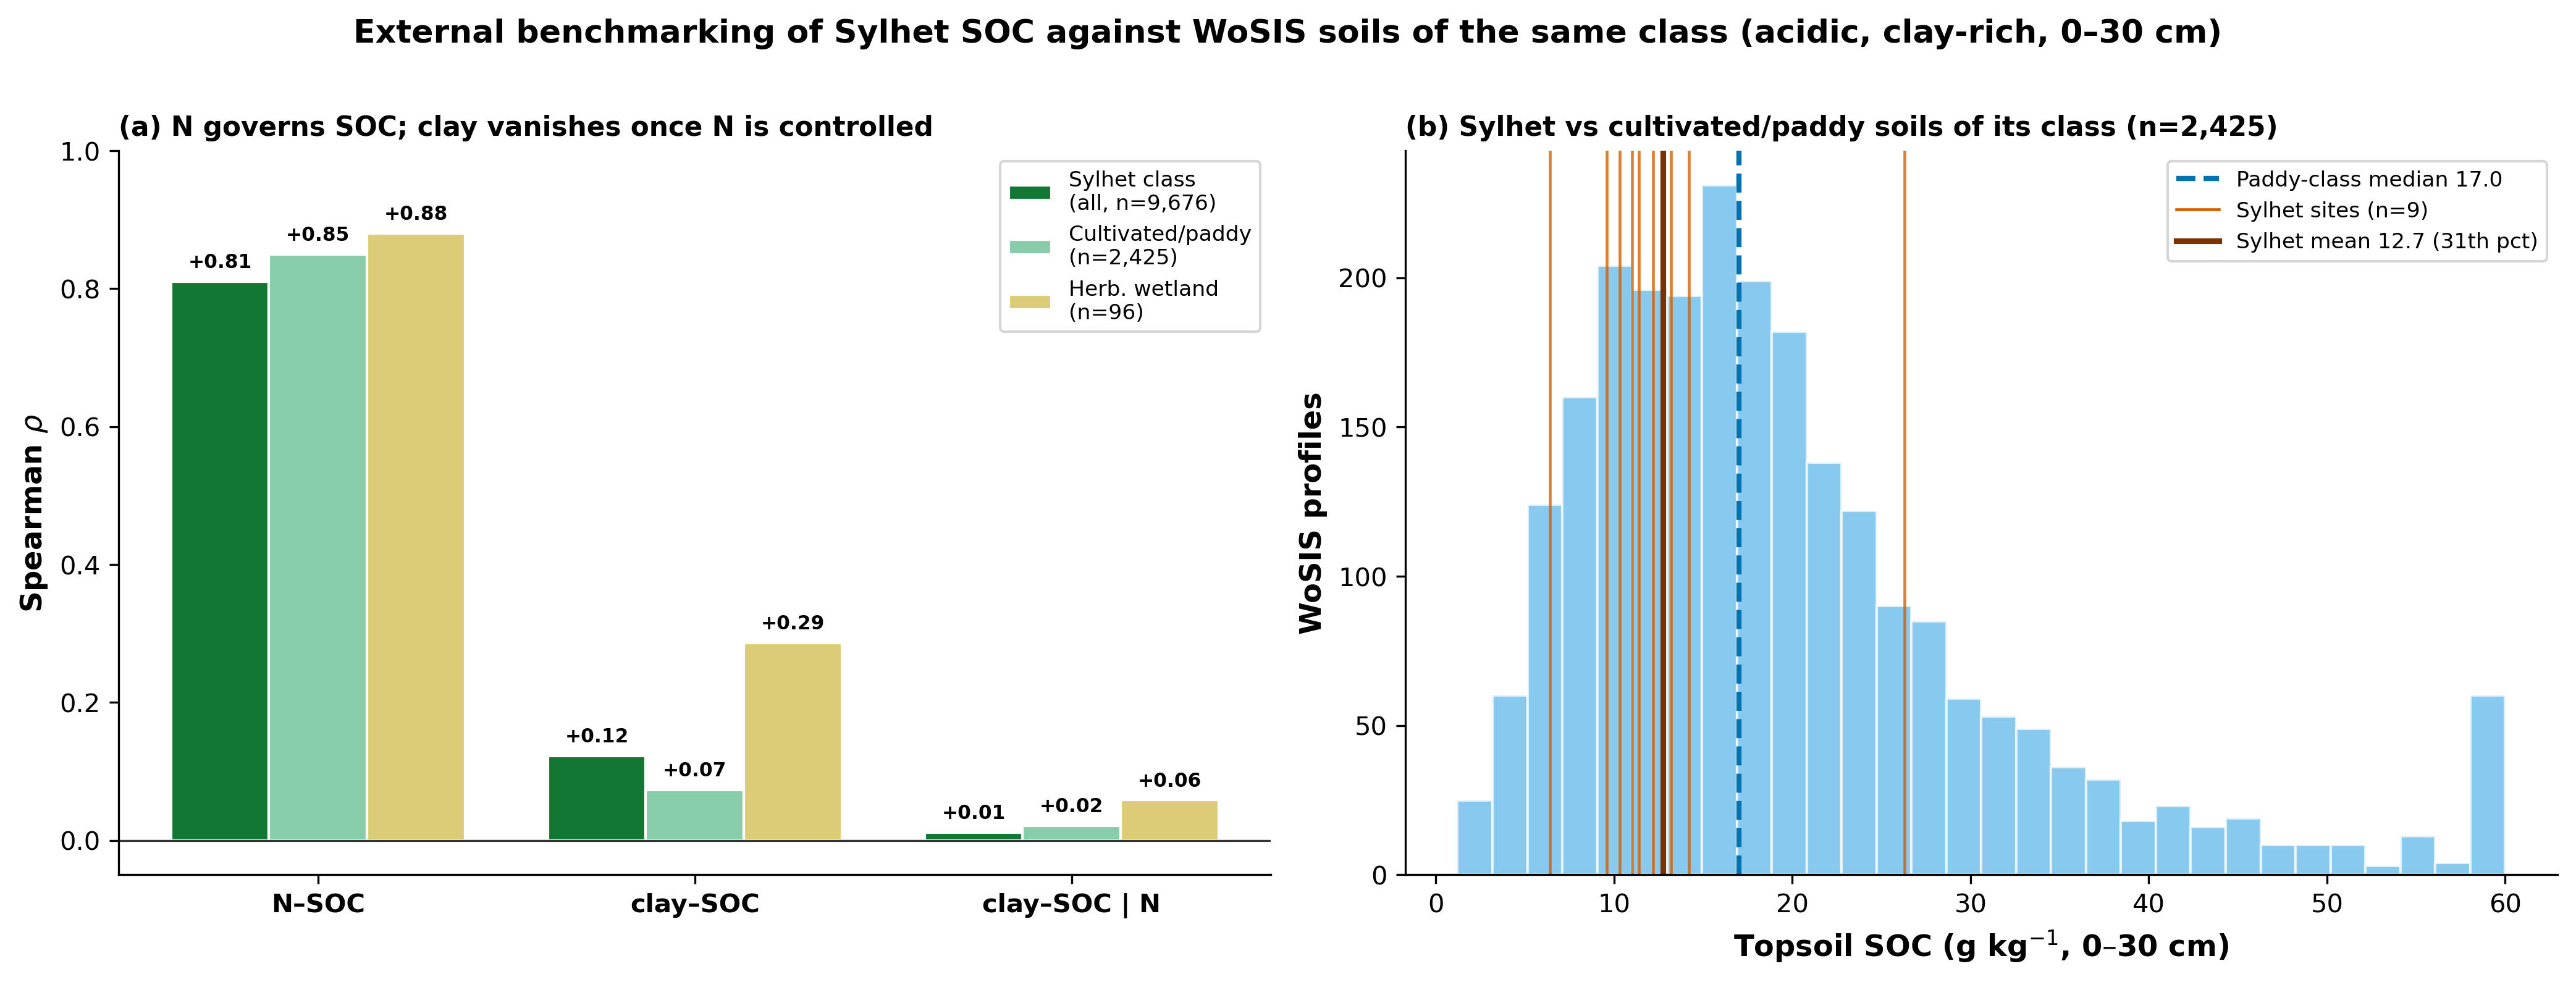
\includegraphics[width=0.95\textwidth]{Fig12_WoSIS_benchmark.png}
\caption{External benchmarking against WoSIS soils of the Sylhet class (acidic, clay-rich,
0--30~cm). (a) SOC--property Spearman effect sizes (N--SOC, clay--SOC, and clay--SOC partialled
on N) for the soil class and its Copernicus land-cover subsets (cultivated/paddy $n=2{,}425$;
herbaceous wetland $n=96$): nitrogen dominates throughout, and clay's weak effect collapses once
nitrogen is controlled. (b) Topsoil SOC distribution of cultivated/paddy soils of the class
($n=2{,}425$) with the nine Sylhet sites overlaid; Sylhet sits near and somewhat below the median.}
\label{fig:wosis}\end{figure}

%% ============================================================
\section{Discussion}
\label{sec:discussion}

\subsection{A wetland under warming, drying and agricultural intensification}
The robust environmental signals are a significant warming (dry-season LST $+0.55\,^{\circ}$C
decade$^{-1}$, $p=0.015$; ERA5-Land air temperature $+0.18\,^{\circ}$C decade$^{-1}$, $p<0.001$),
a multi-decadal \emph{drying} evident in ERA5-Land root-zone soil moisture ($p=0.02$) and
precipitation ($p=0.02$), a significant dry-season greening ($+22$\%, Mann--Kendall $p<0.001$)
indicating expanding irrigated Boro rice, and a monotonic $76$\% expansion of built-up area
(2017--2024, $p<0.01$). An important distinction underlies the drying result. The large
year-to-year swings in the open-water and flood-prone \emph{classes} are seasonal hydroperiod
and image-timing effects (the combined water$+$wetland footprint is constant to within
$\sim$1\% CV; Section~\ref{subsec:lulc-change}), and the optical water index NDWI is likewise
confounded ($r=-0.97$ with greenness)---so the satellite products cannot, by themselves,
demonstrate drying, and we do not infer it from them. The drying signal instead comes from
independent reanalysis: soil moisture and rainfall are falling even though the wet-season
inundated extent appears stable. This reconciles the apparent paradox in earlier framings---a
basin can become drier (lower soil water, less rain, warmer) without its monsoon footprint
shrinking. The defensible picture is therefore one of \emph{warming, drying and agricultural
intensification}. The plausible mechanism for SOC loss accordingly
shifts: warmer soils raise decomposition rates, and intensified dry-season cultivation
(field drainage for Boro, residue export, tillage, and a longer aerobic phase) accelerates
organic-matter turnover \citep{Chen2021}. The warming limb of this mechanism is not merely
assumed: our space-for-time benchmark (Section~\ref{subsec:wosis}) shows that, even within
Sylhet-like warm, wet climates, SOC declines modestly with temperature after nitrogen and
rainfall are controlled---so the basin's measured warming is a credible, if secondary, driver of
SOC loss relative to the dominant organic-matter/nitrogen control. This supports H1 as a \emph{directional}
hypothesis, with the important caveats that LST is a surface proxy, that soil temperature,
decomposition and organic-matter inputs were not measured directly, that hydroperiod remains
unquantified, and that the space-for-time substitution is not a temporal trend; the link to SOC
is strongly suggested but not locally demonstrated.

\subsection{SOC is limited by organic-matter inputs, not by clay (texture)}
Across these nine haors, SOC was unrelated to clay content for every metric tested; the highest
stocks occurred under irrigated Boro--fallow management (Ajmiriganj). Crucially, this clay null
is not a small-sample artifact: benchmarking against $\sim$9{,}700 WoSIS profiles of the same
soil class (Section~\ref{subsec:wosis}) reproduces it---clay's already-weak association vanishes
within the class, while globally, across \emph{all} soils, clay does show a modest positive
association with SOC ($\rho=0.25$). The contrast is the point: in soils where clay is already
abundant (here 30--72\%), the mineral-associated organic-matter pool approaches saturation and
additional clay confers little extra protective capacity, so texture ceases to be the limiting
control \citep{Cotrufo2019,Georgiou2022}. We are deliberately cautious about the complementary
SOC--nitrogen association: because soil N is overwhelmingly organic and C:N ratios are
constrained, SOC and TN are partly coupled by construction, and we therefore read the
association as confirming that SOC here is governed by organic-matter \emph{quantity}---inputs
and management---rather than as evidence that nitrogen is an independent driver. The defensible,
non-trivial conclusion is the absence of a texture control: H2, as a ``finer texture stores more
SOC'' hypothesis, is not supported in this clay-rich, acidic regime. The management implication follows directly: protecting and enhancing
SOC here depends on sustaining organic-matter inputs through flooded, residue-returning rice
systems, not on soil texture.

\subsection{Greening as agricultural intensification}
Dry-season NDVI rose significantly while the classified vegetation \emph{area} (a seasonally
sensitive, year-to-year-noisy quantity) declined modestly. The robust, water-controlled greening
is most plausibly agricultural intensification---the expansion and densification of high-NDVI
dry-season irrigated Boro rice---consistent with regional accounts of Boro expansion in
Bangladeshi wetlands \citep{Mainuddin2021}. We note, however, that we did not independently verify
cropping intensity (e.g.\ against agricultural-census or crop-calendar data), and dry-season
greening can in principle also reflect CO$_2$ fertilization, increased fertilizer use, or improved
cultivars; we therefore present intensification as the most likely driver given the regional
context rather than as a demonstrated cause. The distinction from wetland recovery matters
regardless of mechanism: greenness gains here do not indicate hydrological recovery, and the
drainage, residue export and tillage that accompany intensified dry-season cropping are themselves
plausible drivers of SOC loss rather than gain.

\subsection{Limitations}
\label{subsec:limitations}
% Reviewer E2, E4, comments 1, 34, 40.
Several limitations bound our inferences. (1) \emph{The field dataset is small} ($n=9$ sites,
single 2025 sampling), so all site-level multivariate analyses are exploratory; our more robust
soil inferences rest on the external benchmarking against $\sim$9{,}700 comparable profiles rather
than on the nine sites alone. (2) \emph{The causal chain is not closed locally}: we document
statistically supported environmental pressures (warming, drying, intensification) and a 2025 soil
snapshot, but---because the long-term SOC change is not statistically resolvable here---we do not
demonstrate that these pressures have altered SOC at these specific sites. The driver--SOC link is
inferred from the space-for-time benchmark and the literature, not established locally; this is
therefore a carbon-\emph{vulnerability} assessment, not a measured carbon-\emph{change} study.
(3) \emph{Temporal scope differs across data streams} (SOC 2025/uncertain 1985, indices
1988--2025, LULC 2017--2024, ERA5 1985--2025, GLDAS 2000--2025, GRACE 2003--2016); we therefore
avoid treating them as one continuous record and interpret each on its own window. (4) \emph{The
1985 baseline is secondary reconnaissance data} with screened impossible values, so long-term SOC
change is reported only as uncertain context. (5) \emph{Mechanistic rates were not measured}:
hydroperiod, decomposition, organic-matter inputs and cropping intensity were inferred from
proxies, not quantified directly. (6) \emph{The remote-sensing and reanalysis products are
model-dependent} and partly share inputs. These limitations motivate permanent monitoring plots
with periodic resampling, full-profile sampling, direct hydroperiod measurement, and ground
validation of cropping intensity.

\subsection{Implications and recommendations}
\label{subsec:implications}
These haors store SOCiT of about 31--123 Mg ha$^{-1}$, comparable to other vegetated wetland
and paddy systems and well above typical uplands. The combination of significant warming
($+0.55\,^{\circ}$C decade$^{-1}$), agricultural intensification, and urban expansion places
these stores at risk: warmer soils and longer aerobic, intensively cultivated dry seasons can
accelerate decomposition of historically accumulated carbon, shifting sinks toward sources.
Management priorities that follow directly from our supported findings are: (i) \textbf{retain
the seasonal flood pulse and lengthen anaerobic periods} where Boro intensification is draining
fields, through water-management and floodplain measures; (ii) \textbf{climate-smart Boro
management} (residue return, reduced tillage, optimized flooding) to sustain OM inputs---the
dominant SOC control here; (iii) \textbf{direct urban expansion away from high-SOC haor cores};
and (iv) \textbf{establish long-term SOC, soil-temperature and hydroperiod monitoring}. We frame
the high-yield Boro example (Ajmiriganj) as a promising but single-site indication that
intensification and SOC retention can be compatible, not as a general result.

%% ============================================================
\section{Conclusions}
\label{sec:conclusion}
% Reviewer comment 40 -- rewritten: claims tied to statistics; mechanisms hedged.
Integrating field sampling with multi-decadal remote sensing and reanalysis, this study
characterizes the Sylhet haors as a wetland system under sustained warming, drying and
agricultural intensification. The clearest, statistically supported signals are warming
(dry-season LST $+0.55\,^{\circ}$C decade$^{-1}$, $p=0.015$; ERA5-Land air temperature
$p<0.001$), drying (ERA5-Land root-zone soil moisture and precipitation both declining,
$p=0.02$), a significant dry-season greening ($+22$\%, Mann--Kendall $p<0.001$) attributable to
expanding irrigated Boro rice, and a monotonic $76$\% gain in built-up area over 2017--2024
($p<0.01$). The drying is detected by independent reanalysis rather than by optical water
indices, which here are confounded by the seasonal open-water fraction; notably, the basin dries
(less soil water, less rain, warmer) even though its wet-season inundated footprint appears
stable, so we caution against inferring flood-regime change from inundated-area imagery alone.
Present-day SOC
(0.64--2.63\%; SOCiT 31--123 Mg ha$^{-1}$) was unrelated to soil texture (clay $r=0.04$,
$p=0.93$)---a null reproduced across $\sim$9{,}700 comparable soils and consistent with
mineral-associated-carbon saturation in these already clay-rich soils---and instead scaled with
organic-matter quantity, implying that inputs and management, not clay protection, set carbon
storage here. A comparison with a cleaned historical baseline suggests SOC has
declined at most sites, but this signal is not statistically significant and is sensitive to
uncertain baseline values, so it should be regarded as a hypothesis for targeted future
monitoring rather than an established trend. We refrain from attributing SOC change to a
single mechanism: hydroperiod, decomposition and OM-input rates were not directly measured.
The practical message is that safeguarding carbon in these haors depends chiefly on
maintaining the seasonal flood regime and OM-returning rice management, supported by long-term
monitoring---a framework transferable to other data-poor South and Southeast Asian wetlands.

%% ============================================================
\section*{CRediT authorship contribution statement}
\textbf{Md Jashim Uddin:} Supervision, Investigation, Field sampling, Project administration,
Writing -- review \& editing. \textbf{Md Rakib Hasan:} Conceptualization, Methodology,
Software, Investigation, Data curation, Writing -- original draft, Visualization.
\textbf{Fazla Zawadul Arabi:} Investigation, Data curation. \textbf{Anomita Faiz:}
Writing -- review \& editing. \textbf{Antara Fairuz:} Writing -- review \& editing.
\textbf{Arafat Rahman:} Investigation, Data curation, Formal analysis.

\section*{Declaration of competing interest}
The authors declare no competing financial interests or personal relationships.

\section*{Acknowledgements}
This research was funded by the University Grants Commission (UGC). The authors acknowledge
the Department of Soil, Water and Environment, University of Dhaka, for laboratory and
logistical support. We acknowledge the Soil Resource Development Institute (SRDI) for the
historical reconnaissance soil-survey data used as the 1985 baseline.

\section*{Data availability}
Datasets are available from the corresponding author on request. Remote-sensing data are from
Google Earth Engine (Landsat, Sentinel-2) and ESA CCI.

\bibliographystyle{elsarticle-harv}
\bibliography{references}

\end{document}
